% This is samplepaper.tex, a sample chapter demonstrating the
% LLNCS macro package for Springer Computer Science proceedings;
% Version 2.20 of 2017/10/04
%
\documentclass[runningheads]{llncs}
%
\usepackage{graphicx}
\usepackage{amsmath}
\usepackage{cite}
\usepackage{listings}
\usepackage{algorithm}
\usepackage{algorithmicx}
\usepackage{algpseudocode}
\usepackage{setspace}
\usepackage{booktabs} %三线表
\usepackage{array}    %指定列宽并居中
\usepackage{float}
\usepackage{multirow} %多行合并
% Used for displaying a sample figure. If possible, figure files should
% be included in EPS format.
%
% If you use the hyperref package, please uncomment the following line
% to display URLs in blue roman font according to Springer's eBook style:
% \renewcommand\UrlFont{\color{blue}\rmfamily}

\begin{document}
%
%define vars
\def \toolname {}
%
\title{Orchestrating Smart Home Services from Natural Language Instructions - A Framework based on Runtime Knowledge Graph}
%
%\titlerunning{Abbreviated paper title}
% If the paper title is too long for the running head, you can set
% an abbreviated paper title here
%
\author{Xing Chen\inst{1} \and
Liwei Shen\inst{2,3} \and
Zhangying Lin\inst{1} \and
Zhiming Huang\inst{1}}
%
\authorrunning{X. Chen et al.}
% First names are abbreviated in the running head.
% If there are more than two authors, 'et al.' is used.
%
\institute{Fuzhou University, FuZhou, , China \and
School of Computer Science, Fudan University, Shanghai, 200433, China \and
Shanghai Key Laboratory of Data Science, Fudan University, Shanghai, 200433, China}

%
\maketitle              % typeset the header of the contribution
%
\begin{abstract}
The abstract should briefly summarize the contents of the paper in
150--250 words.

\keywords{Smart Home  \and End-user Manipulation \and Knowledge Graph.}
\end{abstract}
%
%
%
\section{Introduction}\label{sec:introduction}

With the continuous development of smart home infrastructure, smart home has gradually entered a new period characterized by smart services. A large number of complex and heterogeneous intelligent devices cooperate with each other to form a massive, intelligent and integrated context-aware intelligent home service. By analyzing the environment, state and even emotional information of the user, the device can make corresponding preparations with foresight. For example, it can provide accurate temperature control, air purification and other services according to the changes of the situation of the service object. It is a typical representative of intelligent home application. At present, smart home services tend to adopt end-user Programming. End-user Programming can reduce the learning process of Programming language for non-professionals, enabling non-professional users to create, modify or extend components at certain points in the system. Users can customize personalized intelligent home scene services according to their unique needs. To support end-user Programming, you need an infrastructure to control and coordinate devices. However, developing such an infrastructure in a smart home environment presents a number of technical challenges:

$(1)$Most devices do not expose their operating interfaces, making it impossible for end users to complete their programming. In addition, there are differences in brand and function of devices, providing different ways of data reading and function calling, which brings great complexity to device interaction and collaboration.

$(2)$The service needs to meet the needs of personalized scenarios. The differences in devices, types of services and spatial attributes of the scenarios make the interaction between services flexible, and at the same time bring great difficulties to the code logic writing of integrating these services.

In addition, end-user Programming needs to be able to effectively interpret user instructions. Knowledge graph is used to describe the concepts, entities, events and their relationships in the objective world. It can be used to describe the situational knowledge of the smart home, act as a bridge between system requirements and system implementation, and map users' instructions described in natural language to specific devices and services. Two challenges remain:	

$(1)$Knowledge graph is difficult to represent changes in smart home situations. Knowledge graph can organize structured data and represent knowledge with entities and relationships. However, the representation of situational knowledge requires knowledge graph to be able to perceive real-time scene information, while existing knowledge graph technologies are difficult to reflect real-time changes of data.

$(2)$Oriented to personalized service needs, it is necessary to conduct accurate reasoning on knowledge graph considering constraints of device type, location and other dimensions, so it is necessary for knowledge graph to have broader knowledge expression ability. In addition, how to transform the user's natural language instruction into the service capability of the device in the knowledge graph is also an urgent problem to be solved.

This paper proposes a Supporting End-user Programming towards Smart Home Services - A Method based on Runtime Knowledge Graph to solve the problems caused by system complexity in the mapping process of intelligent home service requirements to implementation. The main contributions include:

Firstly, a runtime knowledge graph for smart home is proposed, which represents situational knowledge of users, devices and locations through runtime concepts and relationship examples, so as to realize device interaction and collaboration at the model layer.

Secondly, a natural language-oriented service modeling and execution technology is proposed to generate intelligent home use case scenarios based on the runtime knowledge graph and map the natural language into executable programs on the runtime knowledge graph.

The above method is applied to the actual scenario of smart home, including XX functions on XX devices and XX smart home services. The experimental results show that the user can correctly formulate \% of the smart service at one time, and can formulate \% of the service after feedback.

\section{Overview}\label{sec:overview}

\subsection{Example Scenario of Smart Home}
\begin{figure}
	% \setlength{\belowcaptionskip}{0.1cm}
	\centering
%	\includegraphics[width=0.9\textwidth]{Graph/scenario.png}
    \includegraphics[width=0.9\textwidth]{scenario.png}
	\caption{Example Scenario of Smart Home}
	\label{fig:scenario}
\end{figure}

In this section, we use a scenario shown in Figure~\ref{fig:scenario} to describe the challenges of developing smart home services and the approach used in this article. Scenario includes three locations, which are the sitting room, bedroom and a balcony. Each location sets different intelligent devices, as shown in table 1. For example, the sitting room set air conditioner, smart fan, smart light, PM2.5 Monitor and air purifiers and other device. Scenario include four types of environment status, temperature, humidity, brightness and PM2.5. According to different types of environment condition, intelligent devices can provide monitor, increase, reduce, assign and other services, as shown in table 2. For example, air conditioner can provide temperature monitoring, improvement, reduction and assignment services, air purifier can provide PM2.5 reduction services.

\begin{table}[htbp]
	\caption{Smart Devices in Each Locations}
	\centering  %????
	\label{table1}  % ?????????
	\renewcommand\arraystretch{1.5}  %???????1.5?
	\begin{tabular}{p{3.5cm} p{2.5cm}<{\centering} p{2cm}<{\centering} p{2cm}<{\centering}}  %???????
    \toprule[1.5pt]
	 & Sitting Room & Bedroom & Balcony \\
	\midrule[1.5pt]

	Air Conditioner & 1 & 1 & -\\

	Smart Fan       & 1 & 1 & -\\

	Smart Light     & 1 & 1 & -\\

	PM2.5 Monitor   & 1 & - & -\\

	Air Purifier    & 1 & - & -\\

	Flower Monitor  & - & - & 1\\

	Smart Water Pump& - & - & 1\\

	Smart LED       & - & - & 1\\
	\bottomrule[1.5pt]
	\end{tabular}
\end{table}

\begin{table}[htbp] %????????
	\centering  %????
	\caption{Services Provided by Each Smart Devices}
	\label{table2}
	\renewcommand\arraystretch{1.5}  %???????1.5?
	\begin{tabular}{p{3cm} p{2cm}<{\centering} p{2cm}<{\centering} p{2cm}<{\centering} p{2cm}<{\centering}}  %???????
		
		\toprule[1.5pt]
		& Temperature & Humidity & Brightness & Particulate Matter 2.5 \\
		\midrule[1.5pt]
		
		Air Conditioner & Monitor/Increase/Reduce/Assign & - & - & -\\
		
		Smart Fan       & Monitor/Increase/Reduce/Assign & - & - & -\\
		
		Smart Light     & - & - & Monitor/Increase/Assign & -\\
		
		PM2.5 Monitor   & - & - & - & Monitor\\
		
		Air Purifier    & - & - & - & Reduce\\
		
		Flower Monitor  & - & Monitor & Monitor &\\
		
		Smart Water Pump& - & Increase & - & -\\
		
		Smart LED       & - & - & Increase/Assign & -\\
		\bottomrule[1.5pt]
	\end{tabular}
\end{table}


\begin{table}[htbp]
	\centering  %????
	\caption{Users' Locations and Requirements}
	\label{table3}
	\renewcommand\arraystretch{1.5}  %???????1.5?
	\begin{tabular}{p{2cm}<{\centering} p{2cm}<{\centering} p{2cm}<{\centering} p{2.5cm}<{\centering} p{2cm}<{\centering} p{2cm}<{\centering}}  %???????
		\toprule[1.5pt]
		& Jack & Ken & Sansevieria & Cactus & Lily\\
		& (moving) & (moving) & (sitting room) & (balcony) & (balcony)\\
		
		\midrule[1.5pt]
		
		Temperature & [19$^\circ$C, 26$^\circ$C] & [22$^\circ$C, 26$^\circ$C] & [10$^\circ$C, 35$^\circ$C] & - & -\\ %??^?????\circ????
		
		Humidity    & - & - & - & $>20\%$ & $>60\%$ \\
		
		Brightness  & $>20\%$ & $>20\%$ & $>20\%$ & $>80\%$ & $>70\%$ \\
		
		PM2.5       & $<35\mu g/m^3$ & $<35\mu g/m^3$ & - & - & -\\ %$\mu$
		
		\bottomrule[1.5pt]
	\end{tabular}
\end{table}

The requirements of each user in the scenario are shown in Table~\ref{table3}. User Jack wants indoor temperature to be higher than 19$^\circ$C and lower than 26$^\circ$C(S11), the brightness of the light to be higher than 20\% (S12), PM2.5 to be lower than 35$\mu g/m^3$(S13), user Ken wants indoor temperature to be higher than 22$^\circ$C and lower than 26$^\circ$C(S21), the brightness of the light to be higher than 20\% (S22), and PM2.5 to be lower than 35$\mu g/m^3$(S23).  Sansevieria in the living room lives between 10$^\circ$C and 35$^\circ$C, and the light is stronger than 20\%. Cactus on the balcony lived in the situation where humidity is more than 20\% and the brightness of the light is more than 80\%, while Lily lives in the situation where humidity is more than 60\% and light is more than 70\%.

According to the above requirements, user Jack may send the following instructions to the smart home system in natural language in daily life.

(1) turn on the lights in the bedroom.

(2) what is the PM 2.5 in the sitting room?

(3) when the brightness of the balcony is lower than 80\%, open the smart LED to increase the brightness.

According to the above instructions, the existing smart home system is difficult to deal with. At present, the development of the smart home application is facing many key challenges. First of all, because of the diversity between different brands of devices, there are differences in function, interface. Different brands often provide different ways of data reading and function calls. Because of devices heterogeneous, system can?t integrate all the devices. Therefore the devices cooperate with great complexity in the same scenario. Secondly, there are different types of dynamic service requirements, and the correlation between situational knowledge and intelligent devices needs to be established, which brings great complexity to the writing of service management logic. Because of End-user programming, users can propose personalized scenario of smart home services according to their own needs. The services provided by the system vary with the needs of different end users. The existing smart home system cannot locate to specific scenarios according to the real-time requirements of users, and cannot execute instructions accurately.


\subsection{Approach}
Figure~\ref{fig:overview} is an overview of supporting End-user programming towards smart home services. The method introduces the knowledge graph into the service development process, and realizes the development automation of the situation-aware service through the definition of situation knowledge, the representation of situation knowledge and the modeling and execution of natural language services. The method mainly includes two parts: 1) runtime knowledge graph construction for smart home; 2) service modeling and execution technology for natural language.

\begin{figure}
	% \setlength{\belowcaptionskip}{0.1cm}
	\centering
	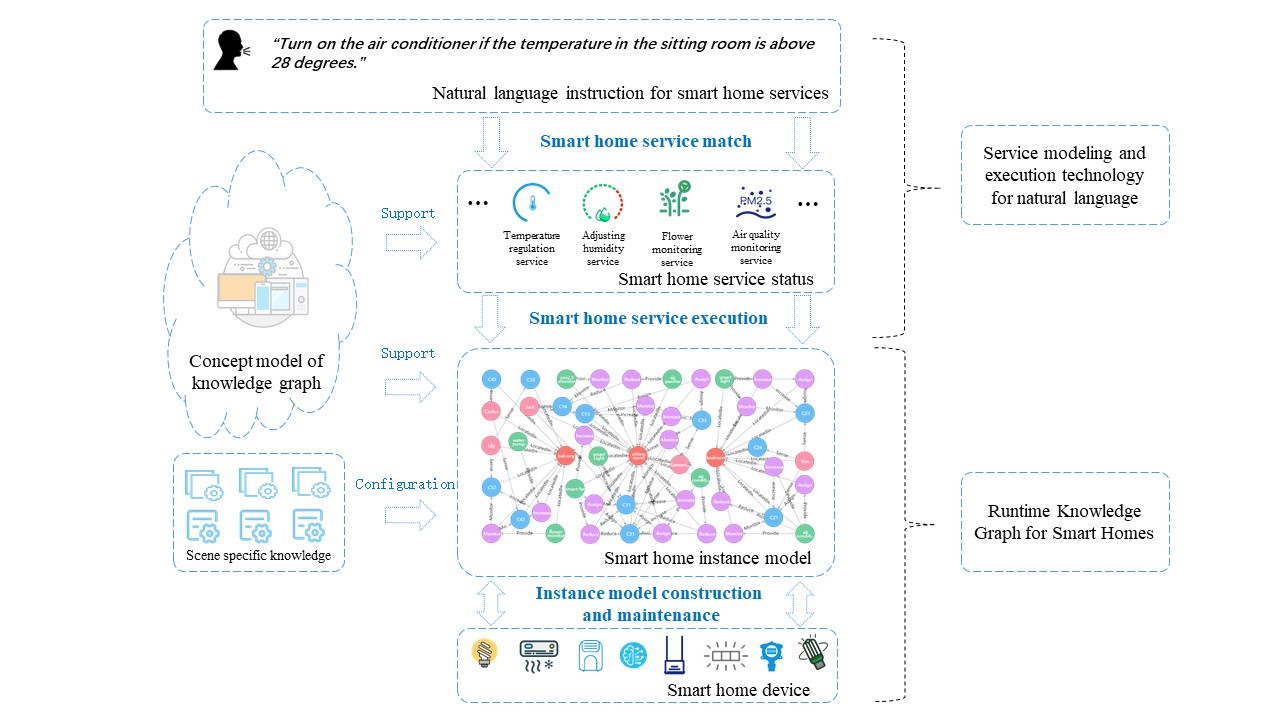
\includegraphics[width=0.9\textwidth]{overview.jpg}
	\caption{Overview of Supporting End-user Programming towards Smart Home Services}
	\label{fig:overview}
\end{figure}

Firstly, the runtime knowledge graph for smart home is proposed. This paper proposes a concept model of knowledge graph for context-aware services of smart home. Concept model of knowledge graph is a knowledge abstraction of the concept level of smart home situational awareness service, describe the concept and the relationship between the abstract elements in the scenario of smart home. The concept model defines the location, user, context, device, services and some concepts in the scenario of smart home. The concept model also defines the relationship such as located in, perception, provide, monitor, increase, reduce, etc. On this basis, the runtime construction method of smart home context-aware service knowledge graph instance model is proposed. The instance model represents smart home situational knowledge through concepts and relational instances, and describes the objective facts in specific scenes. Based on the runtime software architecture model of early work, the runtime construction methods of different types of concepts and relational cases are designed, and the two-way synchronization mechanism between the knowledge map instance model and specific smart home scenarios was established.

Secondly, service modeling and execution technology for natural language is proposed. The runtime knowledge graph for the built smart home generates the corresponding use case description for all the operations or rules on it. When the user sends natural language instructions, it matches the similarity degree with the use case description, so as to find the target operation or rules and automatically decide the device functions to be executed.

Based on the method above, the developer only need to declares the context-oriented knowledge of the scene, configures the mapping relationship between the concept instance and the smart device, and can map the natural language to the executable program on the runtime knowledge graph through the natural language service modeling, and finally formulates the final The service the user needs.

The user can quickly customize the smart home service according to the scene, and can wake up multiple similar devices in the same place to work together. For example, when the temperature needs to be adjusted, the method controls all the devices with temperature adjustment function in the room to meet the requirements of the user. The method can make simple decisions based on instructions from the user. Take an instructions sent by user for example. `Turn on the air conditioner if the temperature in the sitting room is above 28 degrees.' System can infer the information of the current use location based on the current location information of the user in the knowledge graph. The location information is `sitting room'. The system clarifies the instructions to `open the air conditioner in the living room', control the devices at the current location to provide services.


\section{Runtime Knowledge Graph for Smart Home}\label{sec:knowledgegraph}
\subsection{Concept Model of Knowledge Graph of Smart Home}
As shown in Figure~\ref{fig:conceptmodel}, concept model of knowledge graph is a knowledge abstraction of the concept level of smart home situational awareness service, describe the concept and the relationship between the abstract elements in the scenario of smart home.
\begin{figure}
	% \setlength{\belowcaptionskip}{0.1cm}
	\centering
	%	\includegraphics[width=0.9\textwidth]{Graph/scenario.png}
	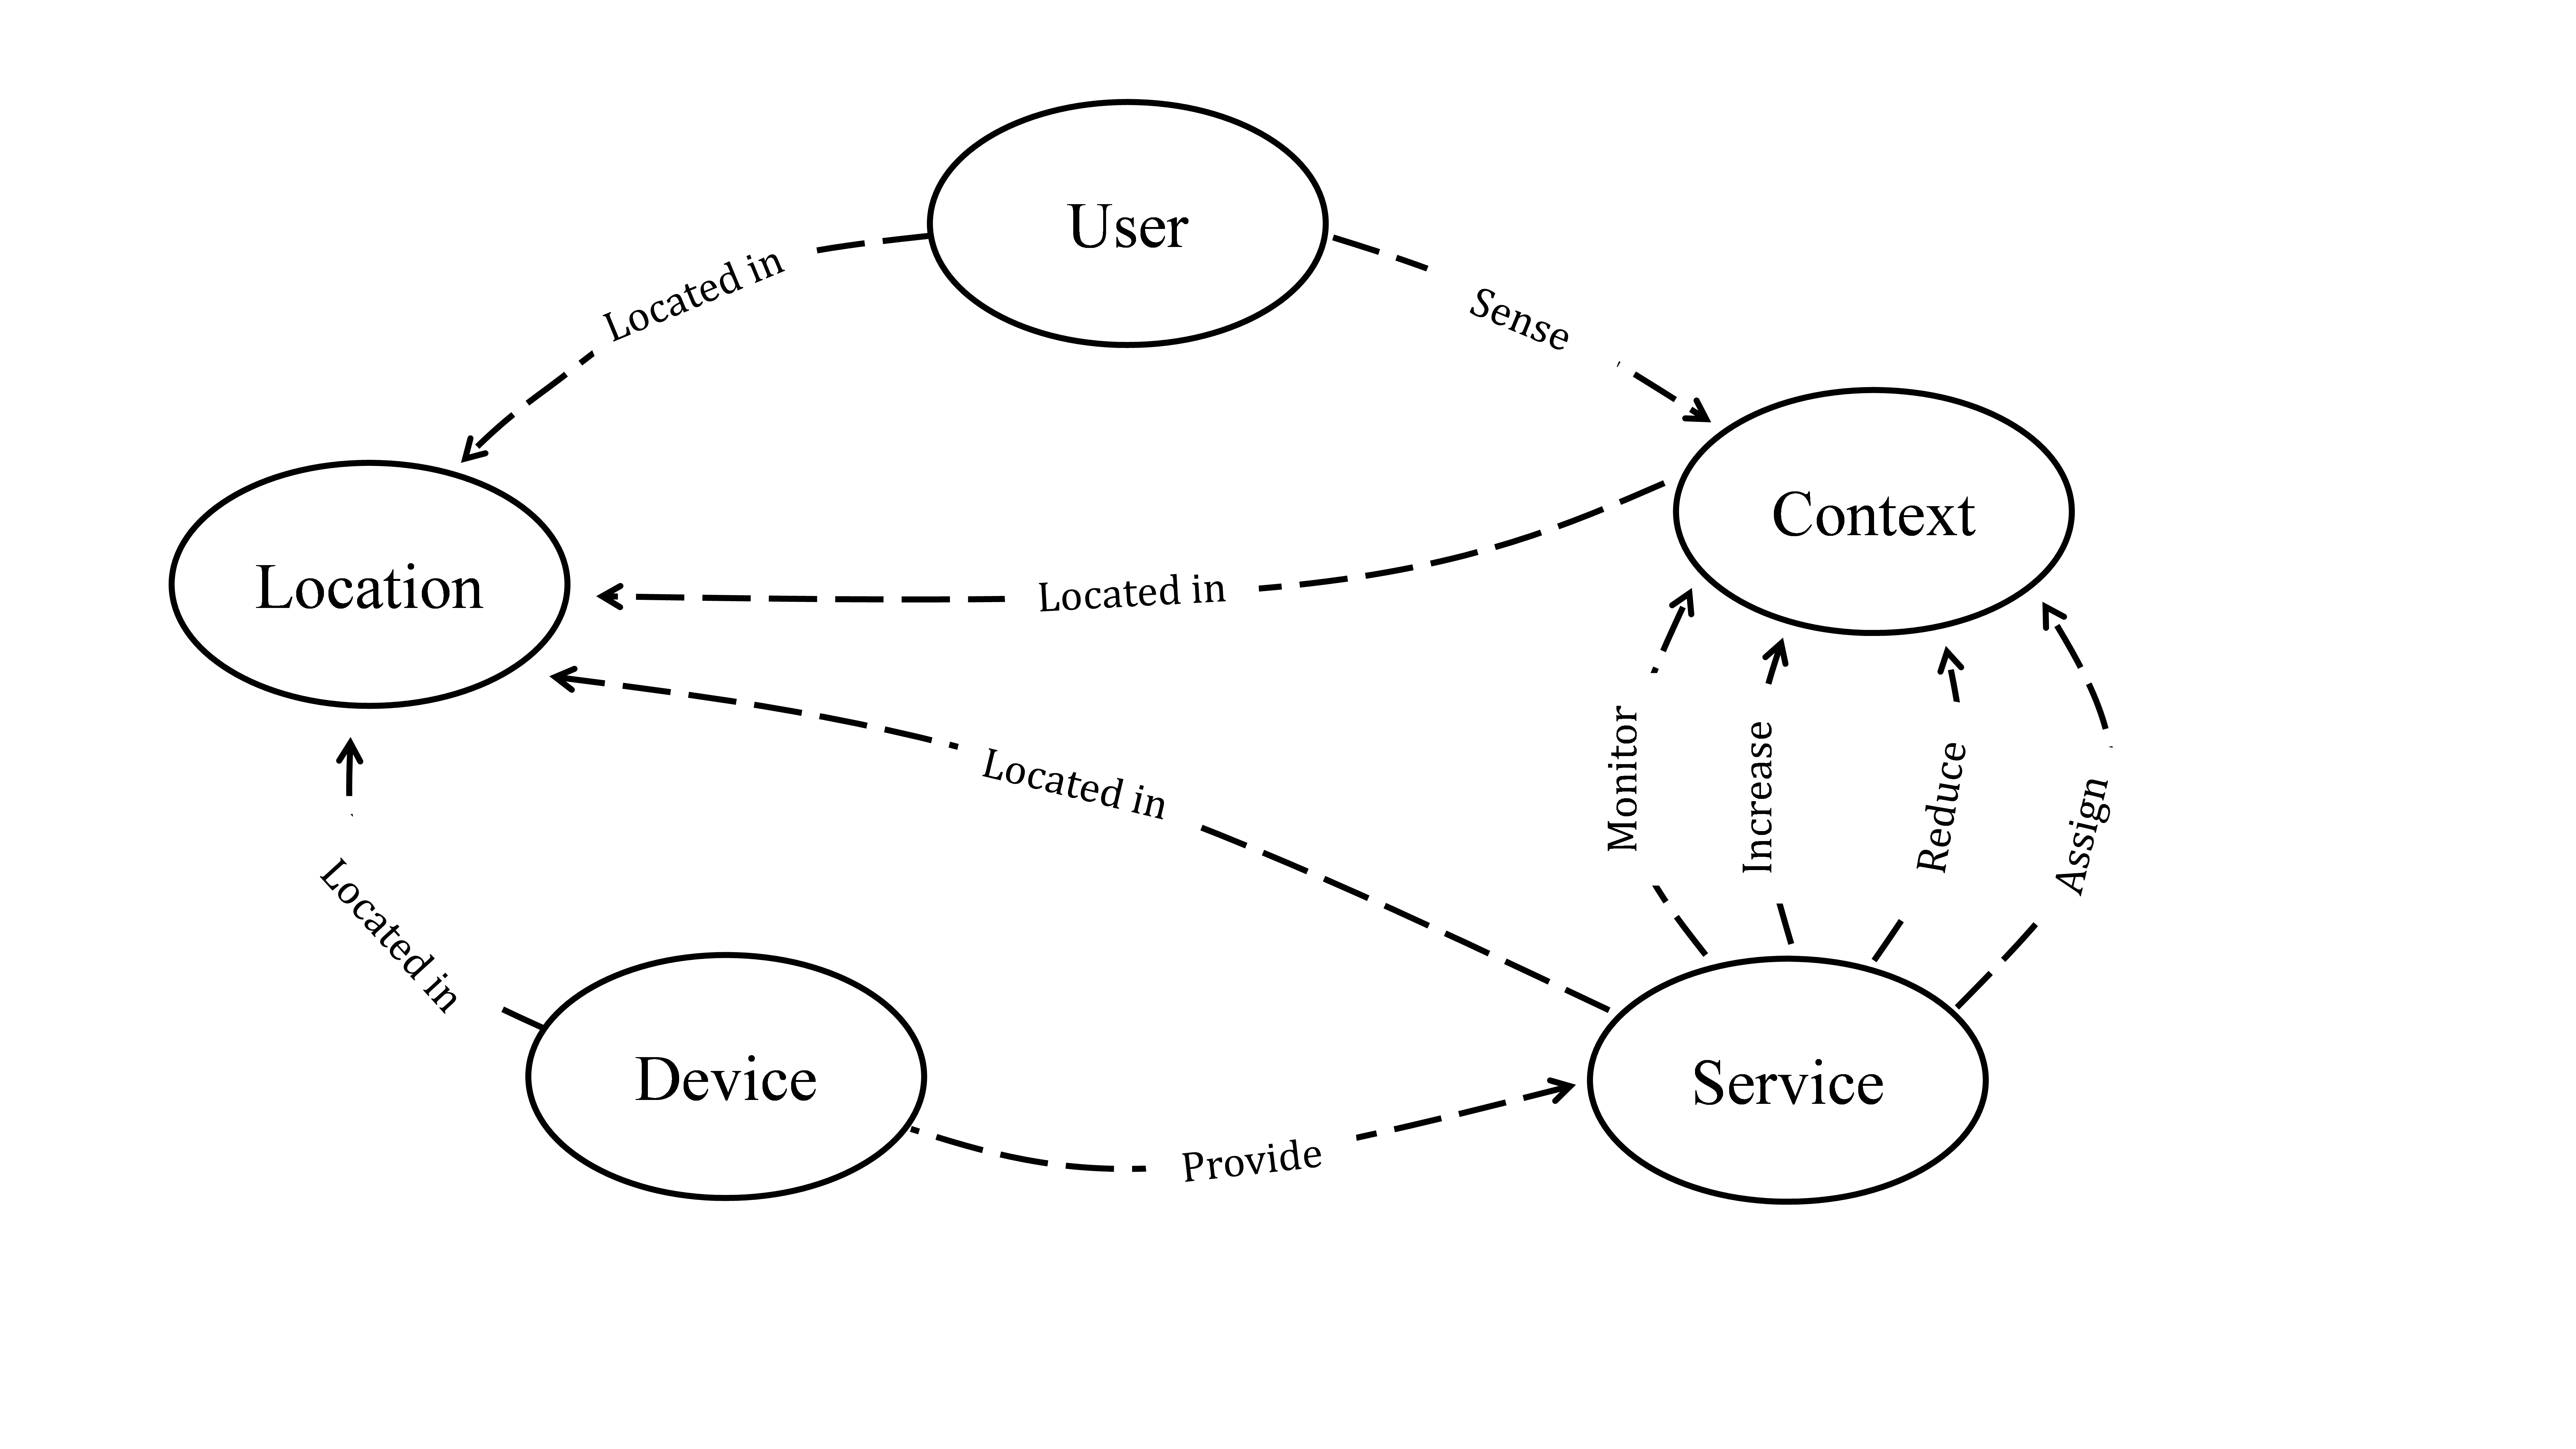
\includegraphics[width=0.9\textwidth]{conceptmodel.png}
	\caption{Concept Model of Knowledge Graph for Context-Aware Services of Smart Home}
	\label{fig:conceptmodel}
\end{figure}
The concept model defines the location, user, context, device, services and some concepts in the scenario of smart home, as shown in Table~\ref{table4}. Wherein, Location represents a specific area, the attribute LName represents the area name. User represents a service object, the attribute UName represents a user name, and the attribute LName represents a user's area. Context represents a certain environment state sensitive to the user. The attribute UName represents the user to which the environment state belongs, the attribute LName represents the area where the environment status is located, the attribute CType indicates the environment status type (for example, light, temperature, etc.). The attribute CValue represents the status value. The attributes RMin and RMax represent the range of state values that need to be met. Device represents a certain smart device. The attribute DName represents the device name. The attribute LName represents the area where the device is located. Status represents whether the device is enabled. The attribute Keyi represents the configuration parameter or system indicator of the device.Service represents a service provided by the smart device to monitor or change the state of the environment. The attribute DName represents the device providing the service, the attribute LName represents the area where the service is located, the attribute CType represents the environment status type of the service monitoring. The attribute Effect represents the effect on the state of the environment, mainly includes four types: Monitor, Increase, Reduce, and Assign. Status represents whether the service is enabled, and SValue represents the environmental status indicator (Monitoring) or service configuration parameters (Assignment).

\begin{table}[htbp]
	\caption{Concepts and Their Attributes in Concept Model of Knowledge Map for Smart Home}
	\centering  %表格居中
	\label{table4}  % 用于索引表格的标签
	\renewcommand\arraystretch{1.5}  %行高变为原来的1.5倍
	\begin{tabular}{|p{2cm}<{\centering}|p{8cm}|}  %指定列宽并居中
		\hline
		Concepts & Concept Attributes \\
		\hline
		Location & $<$ Lname $>$ \\
		\hline		
		User     & $<$ UName,LName $>$\\
		\hline		
		Context  & $<$ UName,LName,CType,CValue ,{RMin,RMax}$>$\\
		\hline		
		Device   & $<$ DName,LName, Status,{Key$_{1}$, Key$_{2}$,…, Key$_{n}$} $>$\\
		\hline		
		Service  & $<$ DName,LName,CType,Effect,Status,SValue $>$\\
		\hline	
	\end{tabular}
\end{table}
The concept model also defines the relationship such as Location in, Sense, Provide, Monitor, Increase, Reduce, Assign and so on , as shown in Figure~\ref{fig:conceptmodel}.

Among them, Located in  $X\xrightarrow[]{Located\,in}L$  represents User U,Context C,Device D,Service S and so on are located in Location L. Sense $U\xrightarrow[]{Sense}C$ represents User U perceives the state of Context C. Provide $D\xrightarrow[]{Provide}S$ represents that Device D provide Service S; Monitor $S\xrightarrow[]{Monitor}C$ represents that Service S is used to monitor the status value of Context C. Increase $S\xrightarrow[]{Increase}C$ represents that Service S is used to increase the state value of Context C. Reduce $S\xrightarrow[]{Reduce}C$ represents that Service S is used to lower the state value of Context C. Assign $S\xrightarrow[]{Assign}C$ represents that Service S is used to change the state value of Context C.

\subsection{Runtime modeling method of smart home knowledge graph instance model}

\subsubsection{Runtime modeling of conceptual instances}

\begin{table}[h]
	\caption{Mapping Rules for Model Operations of Location, User and Context Instances}
	\tiny
	\centering  %????
	\label{table1}  % ?????????
	\renewcommand\arraystretch{1.5}  %???????1.5?
	\newcommand{\tabincell}[2]{\begin{tabular}{@{}#1@{}}#2\end{tabular}}
	\begin{tabular}{p{0.5cm} p{3.6cm}<{\centering} p{3.6cm}<{\centering} p{3.6cm}<{\centering}}  %???????
		\toprule[1.5pt]
		& Location & User & Context \\
		\midrule[1.5pt]
		 List	&\tabincell{c}{List * L $\to$ \{L$_{1}$, L$_{2}$, ..., L$_{n}$\} \\  Get L$_{i}$.properties $\to$ L$_{i}$.properties} 
		 & \tabincell{c}{List * U $\to$ \{U$_{1}$, U$_{2}$, ..., U$_{n}$\} \\  Get U$_{i}$.properties $\to$ U$_{i}$.properties}  & \tabincell{c}{List * C $\to$ \{C$_{1}$, C$_{2}$, ..., C$_{n}$\} \\  Get C$_{i}$.properties $\to$ C$_{i}$.properties}  \\
		\midrule[1.5pt]
		
		 &  &  & Get C$_{i}$.UName $\to$ C$_{i}$.UName\\
		
		    &  &  & Get C$_{i}$.LName $\to$ Get U$_{j}$.LName(($\exists U_{j}$)($U_{j}\xrightarrow[]{Sense} C_{i}$))\\
		
		 Get  & Get L$_{i}$.LName $\to$ L$_{i}$.LName & Get U$_{i}$.UName $\to$ U$_{i}$.UName  & Get C$_{i}$.CType $\to$ C$_{i}$.CType\\
		
		    &  & Get U$_{i}$.LName $\to$ \textbf{RTModel} (Get $T_{i}$.location) & Get C$_{i}$.CValue $\to$ Get S$_{j}$.SValue(($\exists S_{j}$)($S_{j}\xrightarrow[]{Monitor}C_{i}$)$\bigwedge$($S_{j}.Status="On")$))\\
			&  &  & Get C$_{i}$.RMin $\to$ C$_{i}$.RMin \\
			&  &  & Get C$_{i}$.RMax $\to$ C$_{i}$.RMax \\
		\midrule[1.5pt]
			Set       & - & - & -\\
		\bottomrule[1.5pt]
	\end{tabular}
\end{table}

\begin{table}[h]
	
	\tiny
	\centering  %????
	\label{table1}  % ?????????
	\renewcommand\arraystretch{1.5}  %???????1.5?
	\newcommand{\tabincell}[2]{\begin{tabular}{@{}#1@{}}#2\end{tabular}}
	\begin{tabular}{p{0.5cm} p{4.5cm}<{\centering} p{4.5cm}<{\centering} }  %???????
		\toprule[1.5pt]
		& Device & Service  \\
		\midrule[1.5pt]
		List	& \tabincell{c}{List * D $\to$ \{D$_{1}$, D$_{2}$, ..., D$_{n}$\} \\  Get D$_{i}$.properties $\to$ D$_{i}$.properties}  & \tabincell{c}{List * S $\to$ \{S$_{1}$, S$_{2}$, ..., S$_{n}$\} \\  Get S$_{i}$.properties $\to$ S$_{i}$.properties} \\
		\midrule[1.5pt]
		
		&  &   Get S$_{i}$.DName $\to$ S$_{i}$.DName\\%1
		
		& Get D$_{i}$.DName$\to$ D$_{i}$.DName & Get S$_{i}$.LName $\to$ Get D$_{j}$.LName(($\exists D_{j}$)($D_{j}\xrightarrow[]{Provide} S_{i}$))\\%2
		
	   Get & Get D$_{i}$.LName$\to$ D$_{i}$.LName &   Get S$_{i}$.CType $\to$ S$_{i}$.CType \\%3
	    & Get D$_{i}$.Key$_{m}$ $\to$ \textbf{RTModel} (Get D$_{i}$.Key$_{m}$) &   Get S$_{i}$.Effect $\to$ S$_{i}$.Effect \\%4
	    &  &   Get S$_{i}$.Status $\to$ Get D$_{j}$.Key$_{m}$(($\exists D_{j}$)($D_{j}\xrightarrow[]{Provide} S_{i}$))\\%5
	    &  &   Get S$_{i}$.SValue $\to$ Get D$_{j}$.Key$_{n}$(($\exists D_{j}$)($D_{j}\xrightarrow[]{Provide} S_{i}$))\\%6
	   \midrule[1.5pt]
		Set       & Set D$_{i}$.Key$_{m}$ $\to$ \textbf{RTModel} (Set D$_{i}$.Key$_{m}$) & Set S$_{i}$.Status $\to$ Set D$_{j}$.Key$_{m}$(($\exists D_{j}$)($D_{j}\xrightarrow[]{Provide} S_{i}$))\\
				  &  & Set S$_{i}$.SValue $\to$ Set D$_{j}$.Key$_{n}$(($\exists D_{j}$)($D_{j}\xrightarrow[]{Provide} S_{i}$) $\bigwedge$ ($S_{i}.Effect="Assign"$))\\
		\bottomrule[1.5pt]
	\end{tabular}
\end{table}

\paragraph{}
The knowledge graph concept model defines the concepts in the smart home scenes such as location, user, context, device and service. The concept instances are constructed based on the configuration of developers. The two-way synchronization between the concept instance attributes and the scene real-time information is realized through model operation transformation.



Related configurations provided by the developer include scenario-oriented situational knowledge, mapping relationship between concept instances and smart devices, constraints on the context in which the service objects are located, and descriptions of specific locations, users, contexts, devices, and services in the scenario.The scenario-oriented context knowledge provides a set of locations \{L$_{1}$, L$_{2}$, ..., L$_{n}$\} in a specific scenario. The mapping relationship between the concept instance and the smart device provides the device set \{D$_{1}$, D$_{2}$, ..., D$_{n}$ \} in the specific scenario. It provides a set of services \{S$_{1}$, S$_{2}$, ..., S$_{n}$\}, and the relationship between the device and the service; the constraints of the context in which the service object is located describe the set of users \{U$_{1}$, U$_{2}$, ..., U$_{n}$\} in the specific scenario, set of its positioning devices \{T$_{1}$, T$_{2}$, ..., T$_{n}$\}, and the user-sensitive set of environmental states \{C$_{1}$, C$_{2}$,..., C$_{n}$\}.Then, according to the location set L, the user set U, the context set C, the device set D and the service set S, a concept instance of the corresponding type is constructed. Meanwhile, the SM@RT tool[7, 8] is used to construct the smart device and the positioning device. We use runtime model to manage the smart device and positioning device at the model level[9].

The model operation of the concept instance mainly includes three types, namely List, Get, and Set. Among them, “List” represents listing all instances of concept of the type and its attributes, “Get” represents getting the attribute value of concept instance, and “Set” represents setting the attribute value of concept instance. In order to maintain the two-way synchronization of the knowledge map concept instance attribute and the scene real-time information, we define the model operation conversion rule of the concept instance, as shown in Table 5. The location instance L$_{i}$, the value of the attribute LName is from the configuration. User instance U$_{i}$, the value of its attribute UName comes from the configuration.Its attribute LName, which is consistent with the attribute LName of the corresponding device T$_{i}$ in the positioning device runtime model, and the value of the T$_{i}$ is automatically read when the value of the U$_{i}$ attribute LName is read. That is Get U$_{i}$.LName $\to$ \textbf{RTModel} (Get $T_{i}$.location).The context instance C$_{i}$, whose values of the attributes UName and CType are from the configuration. Its attribute LName corresponds to the LName of user instance $U_{j} (U_{j}\xrightarrow[]{Sense} C_{i})$. The value of the U$_{j}$ attribute LName is automatically read when the value of the C$_{i}$ attribute LName is read, that is Get C$_{i}$.LName $\to$ Get U$_{j}$.LName(($\exists U_{j}$)($U_{j}\xrightarrow[]{Sense} C_{i}$)).CValue of context instance is same as the SValue of corresponding service instance $S_{j}\xrightarrow[]{Monitor}C_{i}$.The value of the S$_{j}$ attribute SValue is automatically read when the value of the C$_{i}$ attribute CValue is read, that is Get C$_{i}$.CValue $\to$ Get S$_{j}$.SValue(($\exists S_{j}$)($S_{j}\xrightarrow[]{Monitor}C_{i}$)). Its properties RMin and RMax are from configuration. The attributes DName and LName of the device instance D$_{i}$ are from the configuration. Its attribute Key$_{m}$, which is the same as the attribute Key$_{m}$ of the corresponding D$_{i}$ in the smart device runtime model. When reading/writing the Key$_{m}$ of D$_{i}$ , it will automatically read/write the Key$_{m}$ of D$_{i}$ in the runtime model. That is Get D$_{i}$.Key$_{m}$ $\to$ \textbf{RTModel} (Get D$_{i}$.Key$_{m}$) / Set D$_{i}$.Key$_{m}$ $\to$ \textbf{RTModel} (Set D$_{i}$.Key$_{m}$) .Service instance S$_{i}$, the values of its attributes DName, CType, and Effect, from configuration . The LName of Service instance is the same as the SValue of corresponding device instance. The value of the D$_{j}$ attribute LName is automatically read when the value of the S$_{i}$ attribute LName is read, that is Get S$_{i}$.LName $\to$ Get D$_{j}$.LName(($\exists D_{j}$)($D_{j}\xrightarrow[]{Provide} S_{i}$)). The attribute Status is consistent with the attribute Key$_{m}$ of the device instance D$_{j}$ indicating whether the device is enabled or not. And the value of the D$_{i}$ attribute Key$_{m}$ is automatically read/written when the Status is read/written. That is Get S$_{i}$.Status $\to$ Get D$_{j}$.Key$_{m}$ / Set S$_{i}$.Status $\to$ Set D$_{j}$.Key$_{m}$(($\exists D_{j}$)($D_{j}\xrightarrow[]{Provide} S_{i}$)). The attribute SValue is consistent with the attribute Key$_{n}$ indicating the corresponding environment state in the corresponding device instance D$_{j}$, and the value of the D$_{i}$ attribute Key$_{n}$ is automatically read/written when the value of the S$_{i}$ attribute SValue is read/written. That is Get S$_{i}$.SValue $\to$ Get D$_{j}$.Key$_{n}$ / Set S$_{i}$.SValue $\to$ Set D$_{j}$.Key$_{n}$(($\exists D_{j}$)($D_{j}\xrightarrow[]{Provide} S_{i}$))




\subsubsection{Runtime modeling of relational instances}
\paragraph{}
The knowledge graph conceptual model defines the relationship between concepts in smart home scenarios such as location,  provision, monitoring, improvement, reduction, and assignment, and further defines the runtime construction rules of the relationship instance, as shown in Table 6. When two concept instances satisfy certain preconditions, the relationship instance between them is constructed. Among them, there are instances $X_{i}$ and location instance $L_{j}$ of the user, environment, device, service, etc., and the value of the $X_{i}$ attribute LName is the same as the value of the $L_{j}$ attribute LName. Construct a relationship instance $X_{i}\xrightarrow[]{Located\,in}L_{j}$, indicating that the concept instance $X_{i}$ is located in the location instance $L_{j}$. The relationship instance $U_{i}\xrightarrow[]{Sense} C_{j}$, indicating that the user instance $U_{i}$ senses the environment instance $C_{j}$, the relationship instance $D_{i}\xrightarrow[]{Provide}S_{j}$, indicating that the device instance $D_{i}$ provides the service instance $S_{j}$, both from the configuration information. The service instance $S_{i}$ and the environment instance $C_{j}$ exist, the values of the $S_{i}$ attributes LName, CType and the $C_{j}$ attributes LName, CType are the same, and the $S_{i}$ attribute When the value of Effect is Monitor, the relationship instance $S_{i}\xrightarrow[]{Monitor}C_{j}$ is constructed, indicating that the service instance $S_{i}$ is used to monitor the state value of the environment instance $C_{j}$. The service instance $S_{i}$ and the environment instance exist. $C_{j}$, the value of the $S_{i}$ attribute LName, CType is the same as the value of the $C_{j}$ attribute LName, CType, and the value of the $S_{i}$ attribute Effect is Increase, the relationship instance $S_{i}\xrightarrow[]{Increase}C_{j}$ is constructed, indicating that the service instance $S_{i}$ is used to improve the environment. The state value of the instance $C_{j}$. The existence of the service instance $S_{i}$ and the environment instance $C_{j}$, the values of the $S_{i}$ attributes LName, CType and the values of the $C_{j}$ attributes LName, CType are the same, and the value of the $S_{i}$ attribute Effect is Reduce, constructing the relationship instance $S_{i}\xrightarrow[]{Reduce}C_{j}$, indicating that the service instance $S_{i}$ is used to reduce the state value of the environment instance $C_{j}$. There is a service instance $S_{i}$ and an environment instance $C_{j}$, the values of the $S_{i}$ attributes LName, CType are the same as the values of the $C_{j}$ attributes LName, CType, and the $S_{i}$ attribute Effect When the value is Assign, the relationship instance $S_{i}\xrightarrow[]{Assign}C_{j}$ is constructed, indicating that the service instance $S_{i}$ is used to change the state value of the environment instance $C_{j}$. In addition, since the concept instance attribute is kept in two-way synchronization with the scene real-time information, the relationship instance will be Change as its attribute value changes.

\begin{table}[htbp]
	\caption{Rules for Constructing Relation Instances}
	\centering  %表格居中
	\label{table5}  % 用于索引表格的标签
	\renewcommand\arraystretch{1.5}  %行高变为原来的1.5倍
	\begin{tabular}{|c|c|}  %指定列宽并居中
		\hline
		Relationship instance & Precondition \\
		\hline
		$X_{i}\xrightarrow[]{Located\,in}L_{j}$ & $X_{i}.LName$=$L_{j}.LName$ \\
		\hline		
		$U_{i}\xrightarrow[]{Sense} C_{j}$      & - \\
		\hline		
		$D_{i}\xrightarrow[]{Provide}S_{j}$     & - \\
		\hline		
		$S_{i}\xrightarrow[]{Monitor}C_{j}$     & $S_{i}.LName=C_{j}.LName$ $\Lambda$ $S_{i}.CType=C_{j}.CType$ $\Lambda$ $S_{i}.Effect$ =``Monitor"\\
		\hline		
		$S_{i}\xrightarrow[]{Increase}C_{j}$    & $S_{i}.LName=C_{j}.LName$ $\Lambda$ $S_{i}.CType=C_{j}.CType$ $\Lambda$ $S_{i}.Effect$ =``Increase"\\
		\hline	
		$S_{i}\xrightarrow[]{Reduce}C_{j}$      & $S_{i}.LName=C_{j}.LName$ $\Lambda$ $S_{i}.CType=C_{j}.CType$ $\Lambda$ $S_{i}.Effect$ =``Reduce"\\
		\hline
		$S_{i}\xrightarrow[]{Assign}C_{j}$      & $S_{i}.LName=C_{j}.LName$ $\Lambda$ $S_{i}.CType=C_{j}.CType$ $\Lambda$ $S_{i}.Effect$ =``Assign"\\
		\hline
	\end{tabular}
\end{table}

\subsubsection{Status update for the instance model}
\paragraph{}
In order to maintain the two-way synchronization of the smart home knowledge map instance model and the scene real-time information, the instance model automatically updates the state:

1. Update the concept instance, which in turn is a location instance, a user instance, a device instance, a service instance, and an environment instance.

2. Update the relationship instance, which in turn is the ``Located in" instance, the ``Monitor" instance, the ``Increase" instance, the ``Reduce" instance, and the ``Assign" instance.

3. Repeat execution 1.

\subsection{Knowledge Graph Concept Model Modeling Example}

According to the knowledge of the smart home scenario mentioned above, combined with the example of the smart home scenario in Chapter 2, construct the knowledge graph instance model. According to the example of the smart home scenario in Chapter 2, there are three location instances, corresponding to three regions in the scenario. This section takes some parts of the living room as an example, as shown in Figure~\ref{fig:ch4}.
%\begin{figure}
%	% \setlength{\belowcaptionskip}{0.1cm}
%	\centering
%	%	\includegraphics[width=0.9\textwidth]{Graph/scenario.png}
%	\includegraphics[width=0.9\textwidth]{ch4.png}
%	\caption{Instance Model of the Knowledge Graph for Smart Home}
%	\label{fig:ch4}
%\end{figure}
According to the knowledge of the smart home scenario mentioned above, combined with the example of the smart home scenario in Chapter 2, construct the knowledge graph instance model. According to the example of the smart home scenario in Chapter 2, there are three location instances, corresponding to three regions in the scenario. This section takes some parts of the living room as an example, as shown in Figure 4.
There are two user instances in the living room, which correspond to two service objects in the scene. $U_{1}$ corresponds to Jack, and its attribute LName indicates the area where it is consistent with the corresponding element attribute retention value in the positioning device runtime model. $U_{2}$ corresponds to sansevieria. There are three environment instances, which correspond to the sensitive environment status of each service object in the scenario. For example, the sensitive environment state of Jack ($U_{1}$) is in the same state as the attribute LName of $U_{1}$, and the environment status type is temperature, state value and The attribute SValue of the corresponding service instance maintains the same value, and the constraint range of the state value is [19$^{\circ}$C, 26 $^{\circ}$C]. There are three device instances, which correspond to the Air-Conditioning, Smart Light, and PM2.5 Monitor in the scene. For example, the PM2.5 detector located in the living room has the attribute LName indicating the area, and its attributes $On\_Off$ and PM2.5 are respectively related to the attributes $On\_Off$ and PM2.5 of the corresponding PM2.5 detector device in the smart device runtime model. Consistent. There are 8 service instances, which correspond to the services provided by the smart devices in the scenario; for example, the smart light tube located in the living room has the same value of the LName and the attribute LName of the smart light tube device, and the environmental status type is light intensity. (Brightness), the service type is Monitor, Increse, Assign, whose attribute Status is consistent with the attribute $On\_Off$ of the corresponding device instance, and the attribute SValue and the attribute Brightness of the corresponding device instance are maintained. Consistent.

\section{Modeling and Execution}\label{sec:execution}
Based on the runtime knowledge graph, for all operations or rules thereon, the system generates its corresponding usage description. When the user sends the natural language instruction, it matches the usage description by similarity match to find the target operation or rule.

\subsection{Usage scenario and its corresponding program instructions}
In order to let readers understand the capabilities of the system, combined with the usage scenario in Section 2, this section introduces the types of program instructions based on the runtime knowledge graph.

\subsubsection{Simple operation}
\paragraph{}
Jack can send natural language commands of the ``simple operation" for devices or environments in the scenario. For example, ``Turn on the lights in the bedroom" and ``Increase the temperature in the living room." The program instructions corresponding to the above instructions are divided into operations on the device and operations on the service. The instructions which are operated on device are Set $D_{i}.Status$ to on/off and Set $D_{i}.Keym$ to X. The instructions which are operated on service are Set $S_{i}.Status$ on/off and Set SValue to X. As for natural language commands ``Turn on the lights in the bedroom", the program instructions corresponding to it is “Set $D_{i}.Status$ to on”. $D_{i}.DName$ is Smart Light. For Natural language commands ``Increase the temperature in the living room", the program instructions corresponding to it is ``Set $S_{i}.Status$ to X". $S_{i}.CType$ is temperature.

\subsubsection{Quantitative query}
\paragraph{}
Ken uses the Virtual Assist's Quantitative Query feature to get device attribute values or environmental status values. For example, Ken asks “What is the temperature of the air conditioner?” The temperature value set by the air conditioner can be obtained. By proposing “What is the PM 2.5 of the living room?”, the service of monitoring the living room PM2.5 is turned on, thereby calling the monitoring function of the corresponding device. The program instructions corresponding to the above instructions are divided into two types: device operation and environment operation. The instructions for device operation are: Get $D_{i}.Status$ / Get $D_{i}.Key_{m}$.The instruction for the environment operation is: Get Ci.CValue. Natural language command “What is the temperature of the air conditioner?”  is “Get $D_{i}.Key_{m}$” in the corresponding program command, $D_{i}.DName$ is Air conditioner. Natural language command “What is the PM 2.5 of the living room?” is “Get Ci.CValue” in the corresponding program command, Ci.LName is sitting room.

\subsubsection{Rule setting}
\paragraph{}
The cactus on the balcony needs to survive in a situation where the humidity is greater than 20\% and the light is stronger than 80\%. Depending on the environmental status values, different simple operations need to be triggered. Therefore, the virtual assistant needs to monitor the humidity and brightness of the balcony. When the humidity of the balcony is lower than 20\%, the Smart Water Pump is opened. When the balcony light intensity is less than 80\%, turn on the smart LED to increase the brightness. The program instructions corresponding to the rule settings are as follows: $C_{j}.CValue$ \textgreater X $\mid$  $C_{j}.CValue$ \textless X $\mid$  Y \textless $C_{j}.CValue$ \textless X $\Rightarrow$ Set $D_{i}.Key_{m}$ to X $\mid$  Set $ D_{i}.Status$ to on/off $\mid$ Set $S_{i}.Status$ to on/off $\mid$ Set $S_{i}.Svalue$ to X. In the cactus smart home instruction ``When the humidity of the balcony is below 20\%, open the Smart Water Pump." $C_{j}.LName$ is Balcony, $C_{j}.CValue$ is the humidity of the balcony, X is 20\%, the service provided by the intelligent water valve is Humidity control, $S_{i}.CType$ is Humidity, $S_{i}.Status$ is on.

\subsection{Usage scenario generation based on knowledge graph instance model}
In order to consider all the cases of the knowledge graph instance model in the target scenario, the corresponding usage scenario is generated for all program instructions that may exist.
\subsubsection{Simple operation}
\paragraph{}
For all device instances and service instances in the knowledge graph instance model, modify their properties and convert them into equivalent use cases, indicating that the program instructions can meet the corresponding conditions, as shown in Table 8. It is divided into four situations: changing the state of the device, changing the properties of the device, changing the state of the service, and changing the properties of the service. For example, in the program instruction ``Set $D_{i}.Status$ to on", $D_{i}.DName$ is air conditioner, $D_{i}.Status$ is on, the corresponding generated sentence is ``Turn on the air conditioner in the sitting room. " Program command ``Set $S_{i}.Status$ off" ", $S_{i}.CType$ is brightness, $S_{i}.Effect$ is reduce, $S_{i}.LName$ is sitting room. The corresponding generated sentence is ``reduce the brightness of sitting room . 


%\begin{table}[]
%	\caption{Usage scenario generation rule for simple operation}
%	\centering  
%	\label{table5} 
%	\renewcommand\arraystretch{2} 
%	\begin{tabular}{|l|l|p{2cm}|l|l|}
%		\hline
%		\multicolumn{1}{|c|}{Object} & \multicolumn{1}{c|}{operating}                                          & \multicolumn{1}{c|}{\begin{tabular}[c]{@{}c@{}}Given\\ condition\end{tabular}} & \multicolumn{1}{c|}{\begin{tabular}[c]{@{}c@{}}Program\\ instruction\end{tabular}} & Corresponding usage scenario                   \\ \hline
%		\multirow{3}{*}{device}      & \multirow{2}{*}{\begin{tabular}[c]{@{}l@{}}Change\\ state\end{tabular}} & \multirow{2}{*}{任意Di}                                                          & \begin{tabular}[c]{@{}l@{}}Set\\ Di. Status to on\end{tabular}                     & Turn on /open Di.DName in the Di.LName         \\ \cline{4-5} 
%		&                                                                         &                                                                                & \begin{tabular}[c]{@{}l@{}}Set\\ Di. Status to off\end{tabular}                    & Turn off /shut down Di.DName in the Di.LName   \\ \cline{2-5} 
%		& \begin{tabular}[c]{@{}l@{}}Change\\ attribute\end{tabular}              & 任意Di,任意Keym                                                                    & \begin{tabular}[c]{@{}l@{}}Set\\ Di.Keym to X\end{tabular}                         & Set/Turn“Keym”of Di.DName in the Di.LName to X \\ \hline
%		\multirow{3}{*}{service}     & \multirow{2}{*}{\begin{tabular}[c]{@{}l@{}}Change\\ state\end{tabular}} & \multirow{2}{*}{任意Si 且Si.Effect = Increase/Reduce}                             & \begin{tabular}[c]{@{}l@{}}Set\\ Si.Status on\end{tabular}                         & Increase/Reduce the Si.CType of Si.LName       \\ \cline{4-5} 
%		&                                                                         &                                                                                & \begin{tabular}[c]{@{}l@{}}Set\\ Si.Status off\end{tabular}                        & Reduce/Increase the Si.CType of Si.LName       \\ \cline{2-5} 
%		& \begin{tabular}[c]{@{}l@{}}Change\\ attribute\end{tabular}              & 任意Si 且Si.Effect = Assign                                                       & \begin{tabular}[c]{@{}l@{}}Set\\ Si.Svalue to X\end{tabular}                       & Set the Si.CType of Si.LName to X              \\ \hline
%	\end{tabular}
%\end{table}


\subsubsection{Quantitative query}
\paragraph{}
For all device instances and service instances in the knowledge graph instance model, the attributes are read and converted into equivalent Usage scenarios. When a certain situation occurs, system need to execute the corresponding operation. It is divided into two situations: Query the status and attributes of the device and query the status of the environment. For example, if the smart light is turned on, the corresponding program command ``Get $D_{i}.Status$", $D_{i}.DName$  is smart light, the corresponding sentence generated is ``Is the smart light on ? "


%\begin{table}[!ht]
%	\caption{Usage scenario generation rule for quantitative query}
%	\centering  
%	\label{table6} 
%	\renewcommand\arraystretch{2}  
%	\begin{tabular}{|l|l|p{3cm}|l|l}
%		\cline{1-4}
%		Event  & Given condition & Program instruction & Corresponding usage scenario  &  \\ \cline{1-4}
%		\multirow{2}{*}{\begin{tabular}[c]{@{}l@{}}Query the status \\ and properties of the device\end{tabular}} & 任意Di            & Get Di. Status                       & Is the Di.DName on/off? | What is the status of Di.DName? &  \\ \cline{2-4}
%		& 任意Di 任意Keym     & What is the Di.Keym of the Di.DName? & What is the Di.Keym of the Di.DName?                      &  \\ \cline{1-4}
%		\begin{tabular}[c]{@{}l@{}}Query the status of \\ the environment\end{tabular}                               & 任意Ci            & Get Ci.CValue                        & What is the Ci.CType in the Ci.LName?                     &  \\ \cline{1-4}
%	\end{tabular}
%\end{table}


\subsubsection{Rule setting}
\paragraph{}
Set the inference rules for each operation, triggering the execution of different simple operations based on the environmental state value constraints. The conditions are as shown in Table 10 , the triggered operation is the same as the simple operation. For example, when the living room temperature is lower than 16 degrees, the temperature of the living room is raised. The corresponding program command is “Cj.CValue < X”, where Cj.LName= sitting room, Cj.CValue is the temperature state value of the living room, X=16 Degree, the simple operation corresponding to the improvement of the living room temperature is ``Set $S_{i}.Svalue$ on", $S_{i}.CType$ is temperature, $S_{i}.Effect$ is increase, $S_{i}.Svalue$ is the temperature service parameter, $S_{i}.LName$ is sitting room, the corresponding sentence is If the temperature in the sitting room is less than 16 degrees, increase the temperature of sitting room .

\begin{table}[!ht]
	\caption{Usage scenario generation rule for Rule setting}
	\centering  
	\label{table7} 
	\renewcommand\arraystretch{2}  
		\begin{tabular*}{\hsize}{|l|l|l|}  
			\hline
			Given condition	& Given condition & Corresponding usage scenario \\
			\hline
			$\forall C_{j}$ & $C_{j}.CValue$ \textgreater X & If the $C_{j}.CType$ is higher than/more than/above X\\
			\hline
			$\forall C_{j}$ & $C_{j}.CValue$ \textless X & If the $C_{j}.CType$ is lower than/less than/below X\\
			\hline
			$\forall C_{j}$ & Y \textless $C_{j}.CValue$ \textless X & If the $C_{j}.CType$ is between Y and X\\
			\hline
		\end{tabular*}
\end{table}

\subsection{Automatic conversion of natural language to program instructions}
When a user sends a natural language instruction, it is similarly matched to the usage description to find the target operation or rule. Simple sentences (including simple operations and quantitative queries) directly match the usage scenario, and the compound sentence (rule setting) is first processed into two simple sentences, and then matched separately.

$$X=(x_{1},x_{2},...,x_{n}) \eqno(1-1)$$
$$X_{i}=\frac{\sum_{j=1}^{n}x_{i}}{n}(i=1,2,...,n) \eqno(1-2)$$

Vectorizing representations of words is the basic operation of text analysis. Word vectors can represent text as a continuous, multidimensional vector. In a colloquial manner, the word vector quantifies sentences that are difficult to express. By converting sentences into numbers, sentences can be calculated and speculated. The word vector technique is equivalent to quantifying words that cannot be expressed, and uses spatial distance to reflect the similarity of two words. The higher the similarity of the two words, the closer the distance in space. The more unrelated the two words, the farther the distance in space. Since the similarity between two words and sentences cannot be directly calculated, it is necessary to use the word vector technique to express the sentence as data first. In this paper, a distributed representation is used to represent a word, and a fixed-length m-dimensional vector is used to express an English character, such as formula (1-1). Adding the number of the corresponding dimension of each sentence of a sentence removes the number of words in the sentence, and obtains the fifty-dimensional vector of the sentence, as in formula (1-2).


In this paper, the cosine similarity method is used to match the user instruction with the usage description. In the xoy coordinate axis, the angle between the two vectors can be used to calculate the cosine value. The smaller the angle, the closer the cosine value is to 1, then the directionality of the two vectors is more consistent and similar. Conversely, the closer the cosine value is to zero, the closer the angle is to $90^{\circ}$, indicating that the two vectors are not similar. Promote to multidimensional space, the greater the distance, the smaller the similarity. The smaller the distance, the greater the similarity. From the above conclusions, it can be known that after the angle between the two sentences is obtained, the calculation of the cosine value can be used to determine the similarity of the individual. The vector a is represented by coordinates $(x_{1}, y_{1})$, the vector b is represented by coordinates $(x_{2}, y_{2})$, and the vector n is represented by coordinates $(x_{n}, y_{n})$.
$$ cos(\Theta) =\frac{\sum_{i=1}^{n}(x_{i} \times  y_{i})}{\sqrt{\sum_{i=1}^{n}{x_{i}}^{2}} \times  \sqrt{\sum_{i=1}^{n}{y_{i}}^{2}}}  \eqno(1-3)$$
Then the similarity of two multidimensional vectors can be calculated by equation (1-3). For a simple sentence, take the top5 with the highest similarity as the final match result. For a compound sentence, the processing is two simple sentences that respectively represent conditions and actions, and respectively match. The result of the compound sentence matching is the respective top5 obtained by matching the conditional sentence and the action sentence respectively, and the Cartesian product is obtained. The 25 instructions after the Cartesian product are calculated again with the original compound instruction, and the top 5 is taken out, and the strategy can guarantee The accuracy of compound sentences does not drop too much.

For example, for the user's simple sentence ``Turn up the brightness." Firstly, according to the runtime knowledge garph to query the current user's location information, and get LNAME as the sitting room, according to the above processing rules, the perfect sentence is ``Turn up the brightness in the sitting room." After the sentence is vectorized, the word vector of the sentence is obtained.

The word vector and the generated usage corpus are used to calculate the similarity one by one, and the top5 results are as follows:

increase the brightness of sitting room .

reduce the brightness of sitting room .

turn the brightness of the smart light in the sitting room to x .

monitor the brightness of sitting room .

set the brightness of sitting room to x .

The top1 matching result with the highest similarity value is ``Increase the brightness of sitting room."The similarity calculation result of the two is 0.98767.
The program command matched by this condition is ``Set $S_{i}.Status$ on", wherein the device of $S_{i}.CType$ is brightness and $S_{i}.Lname$ is sitting room is Smart Light, and then the program instruction is executed based on the runtime knowledge .



\section{Evaluation}\label{sec:evaluation}

We have implemented end-user programming approach and evaluated it to explore the following research questions:

(RQ1) What is the accuracy of the instruction recognize approach and how to improve the accuracy of it? (Chapter 5.1)

(RQ2)To what extent can user programming complexity be reduced by using this end-user programming approach? (Chapter 5.2)

(RQ3)Does our approach have an impact on efficiency in end-user programming? (Chapter 5.3)

\subsection{Accuracy of Program Instruction Conversion}

\subsubsection{Experimental Setup}

\paragraph{}
To evaluate the accuracy of our program instruction conversion method, we use 3 data sets: a Base set, a Paraphrase set and a Scenario set. All together, 2304 sentences are collected, of which 1424 are primitive and 680 are compound.

The instructions in the Base set are generated by the generation rules in Section 4.2. The Base set provides the basic instructions for the Smart Home Service, which enables basic control of various devices and functions. A total of 200 instructions are generated in our Base set which consists of 121 primitive sentences and 79 compound sentences.

The instructions in the Paraphrase set are written by trained labor who are familiar with the devices and functions in this smart home scenarios. The Paraphrase set is used to increase the variety of instructions in order to simulate the user's use of smart home devices in real-world scenarios as much as possible. 1057 sentences are collected, of which 714 are primitive and 343 are compound.

The instructions in the Scenario set are given by the volunteers. They are not familiar with the various devices and functions in this smart home scenarios. And the way they know about the devices and functions in this smart home only through our simple oral description and demonstration. Then volunteers give control instructions which based on their experience and understanding of smart home scenarios. We collected more natural sentences by using this approach. The Scenario set has 1047 instructions, including 710 primitive instructions and 337 compound instructions.

We compare the approach of this paper with the rule based approach [1] and the Almond approach [2] in the accuracy of instructions conversion. The rule based approach establishes series of instructions recognition rules and determines the sentence pattern according to the syntax structure for each instruction. It uses the syntax dependency relationship to find information such as actions, device names, place names and context attributes in the instructions. Finally, according to the defined knowledge inference rules, it matches the device, location, and context in the runtime knowledge graph, thereby mapping the instruction to a specific service that can implement the function.The Almond approach obtains information through Thingpedia entries and use machine learning to train the Thingtalk program and its paraphrase to obtain a semantic parser. Finally, the semantic parser is used to parse the user's instructions to match programs. There is only one result for the rule based approach. We measure if the correct answer is among the top 1, 3, and 5 matches in both our approach and the Almond approach


\subsubsection{Analysis of Results}
\paragraph{}

\begin{figure}[h]
\centering
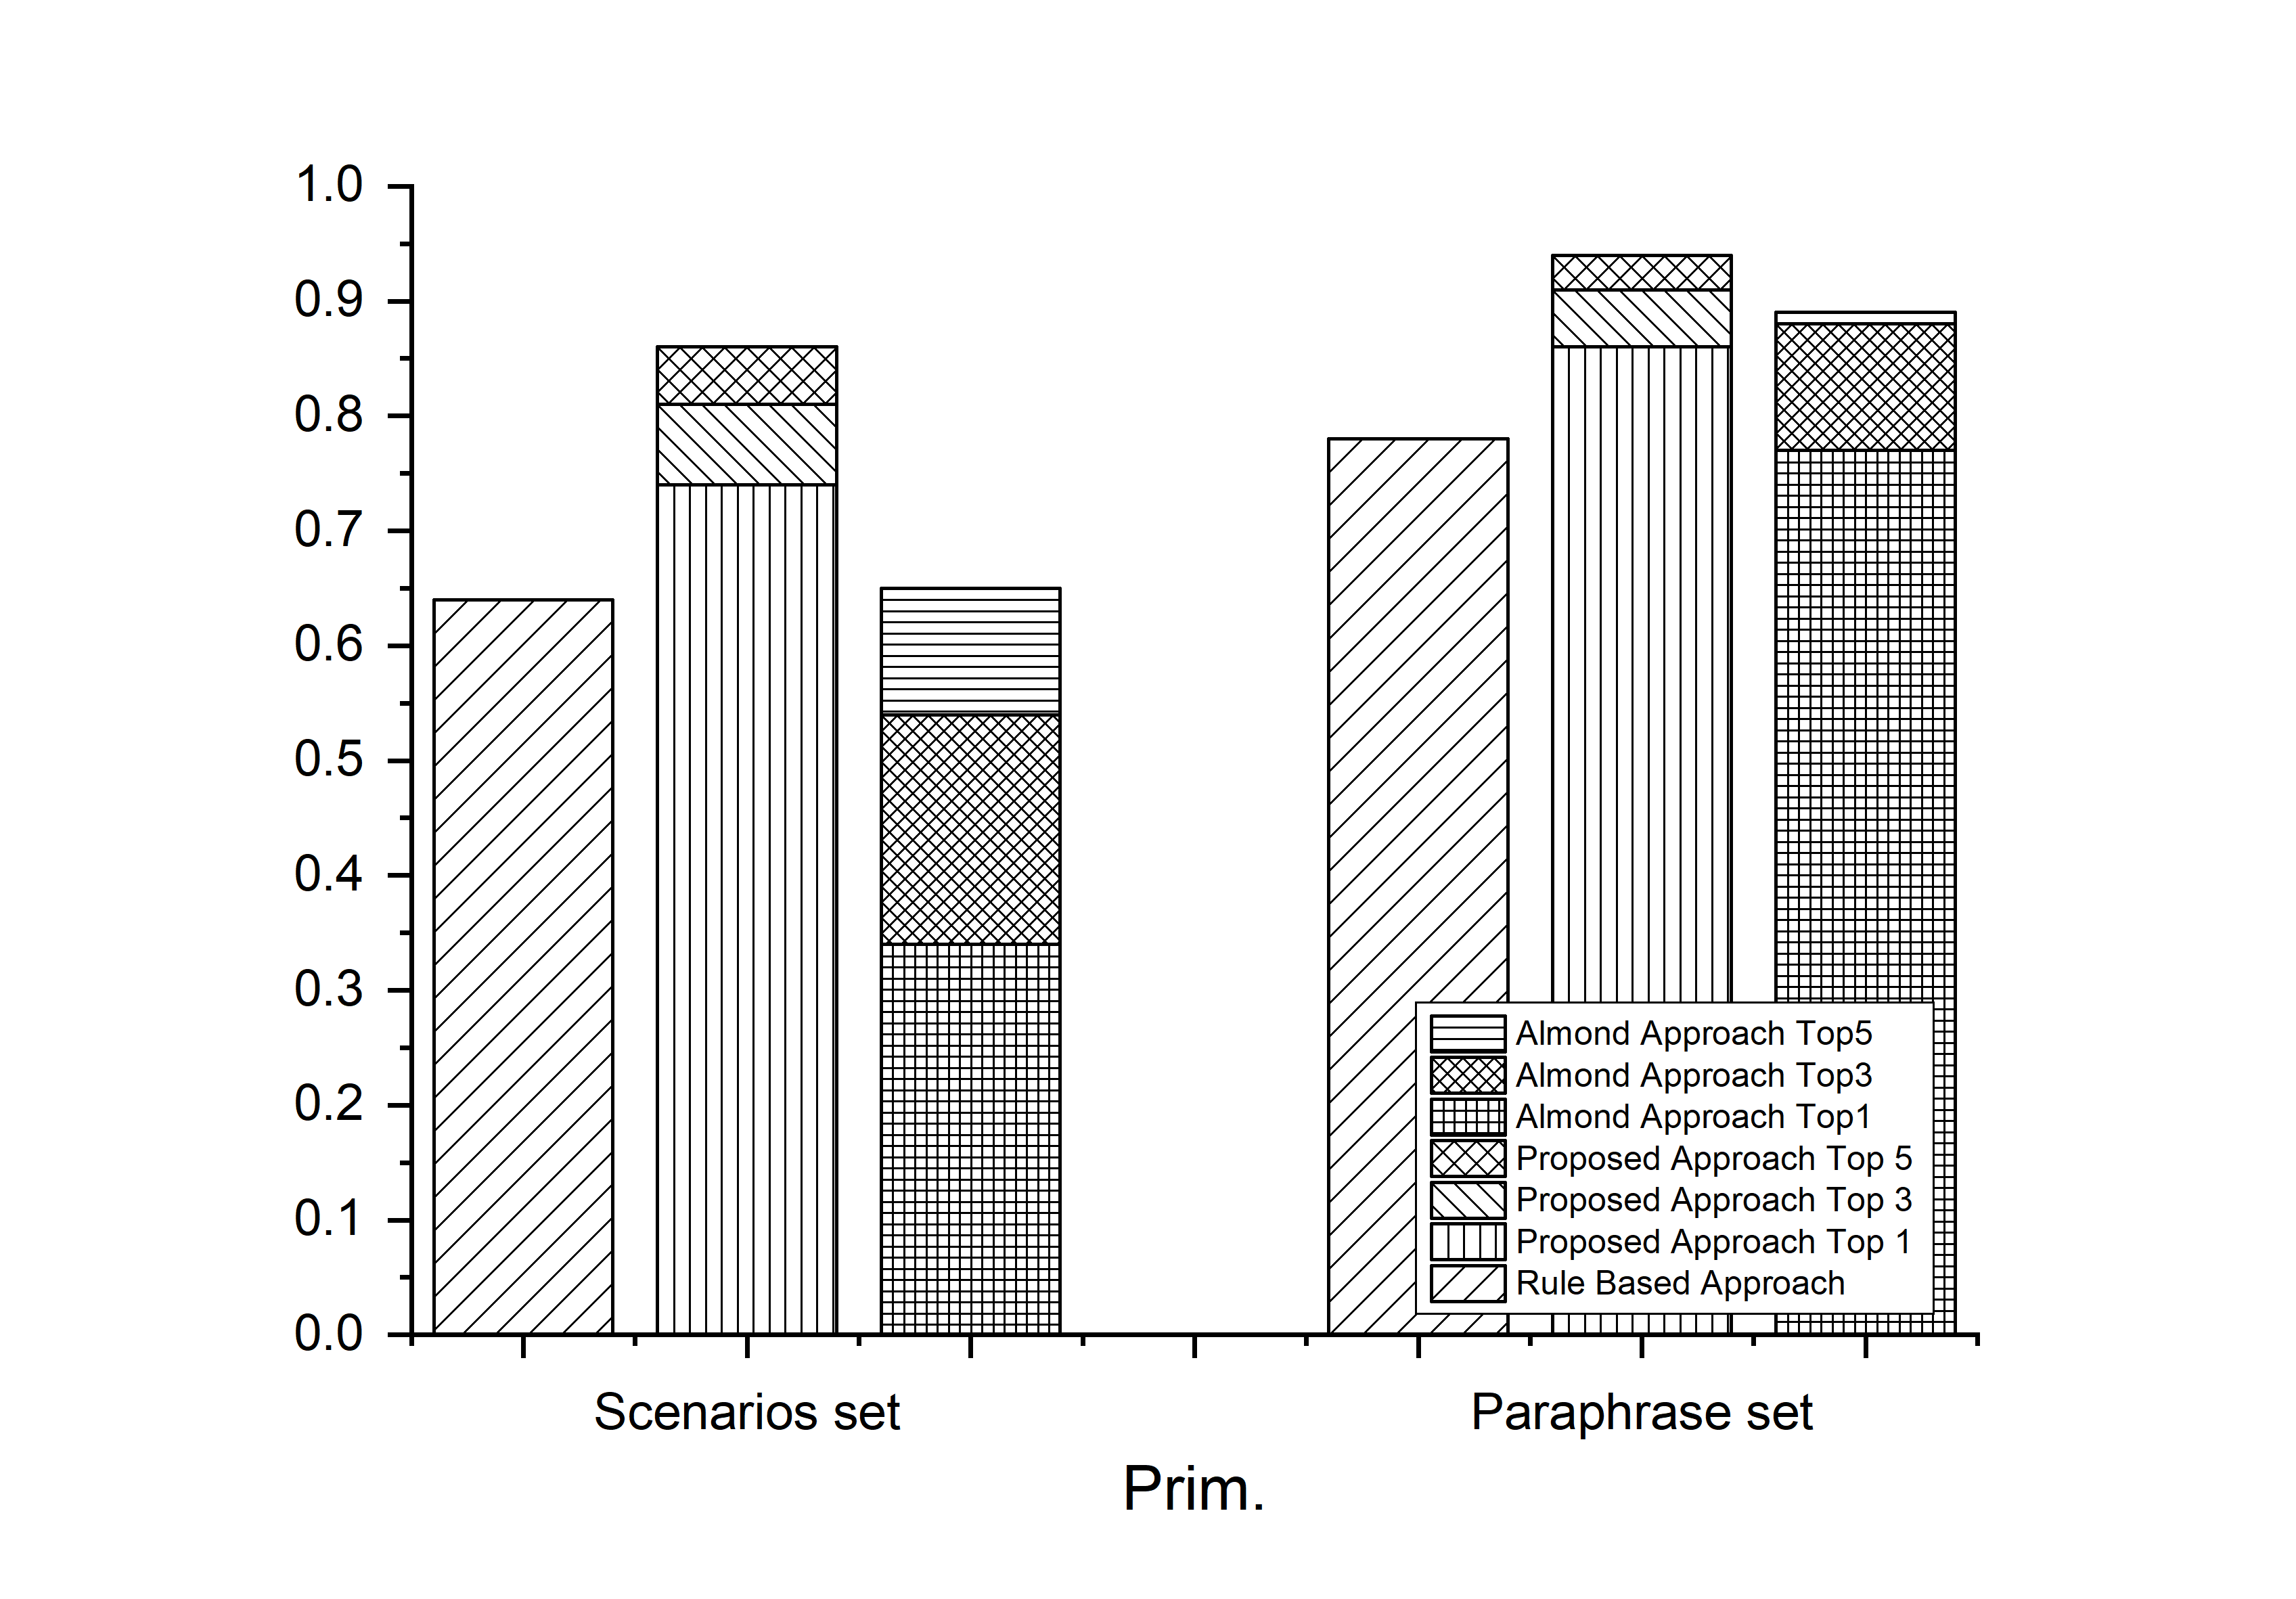
\includegraphics[width = .5\textwidth]{fig5_1.png}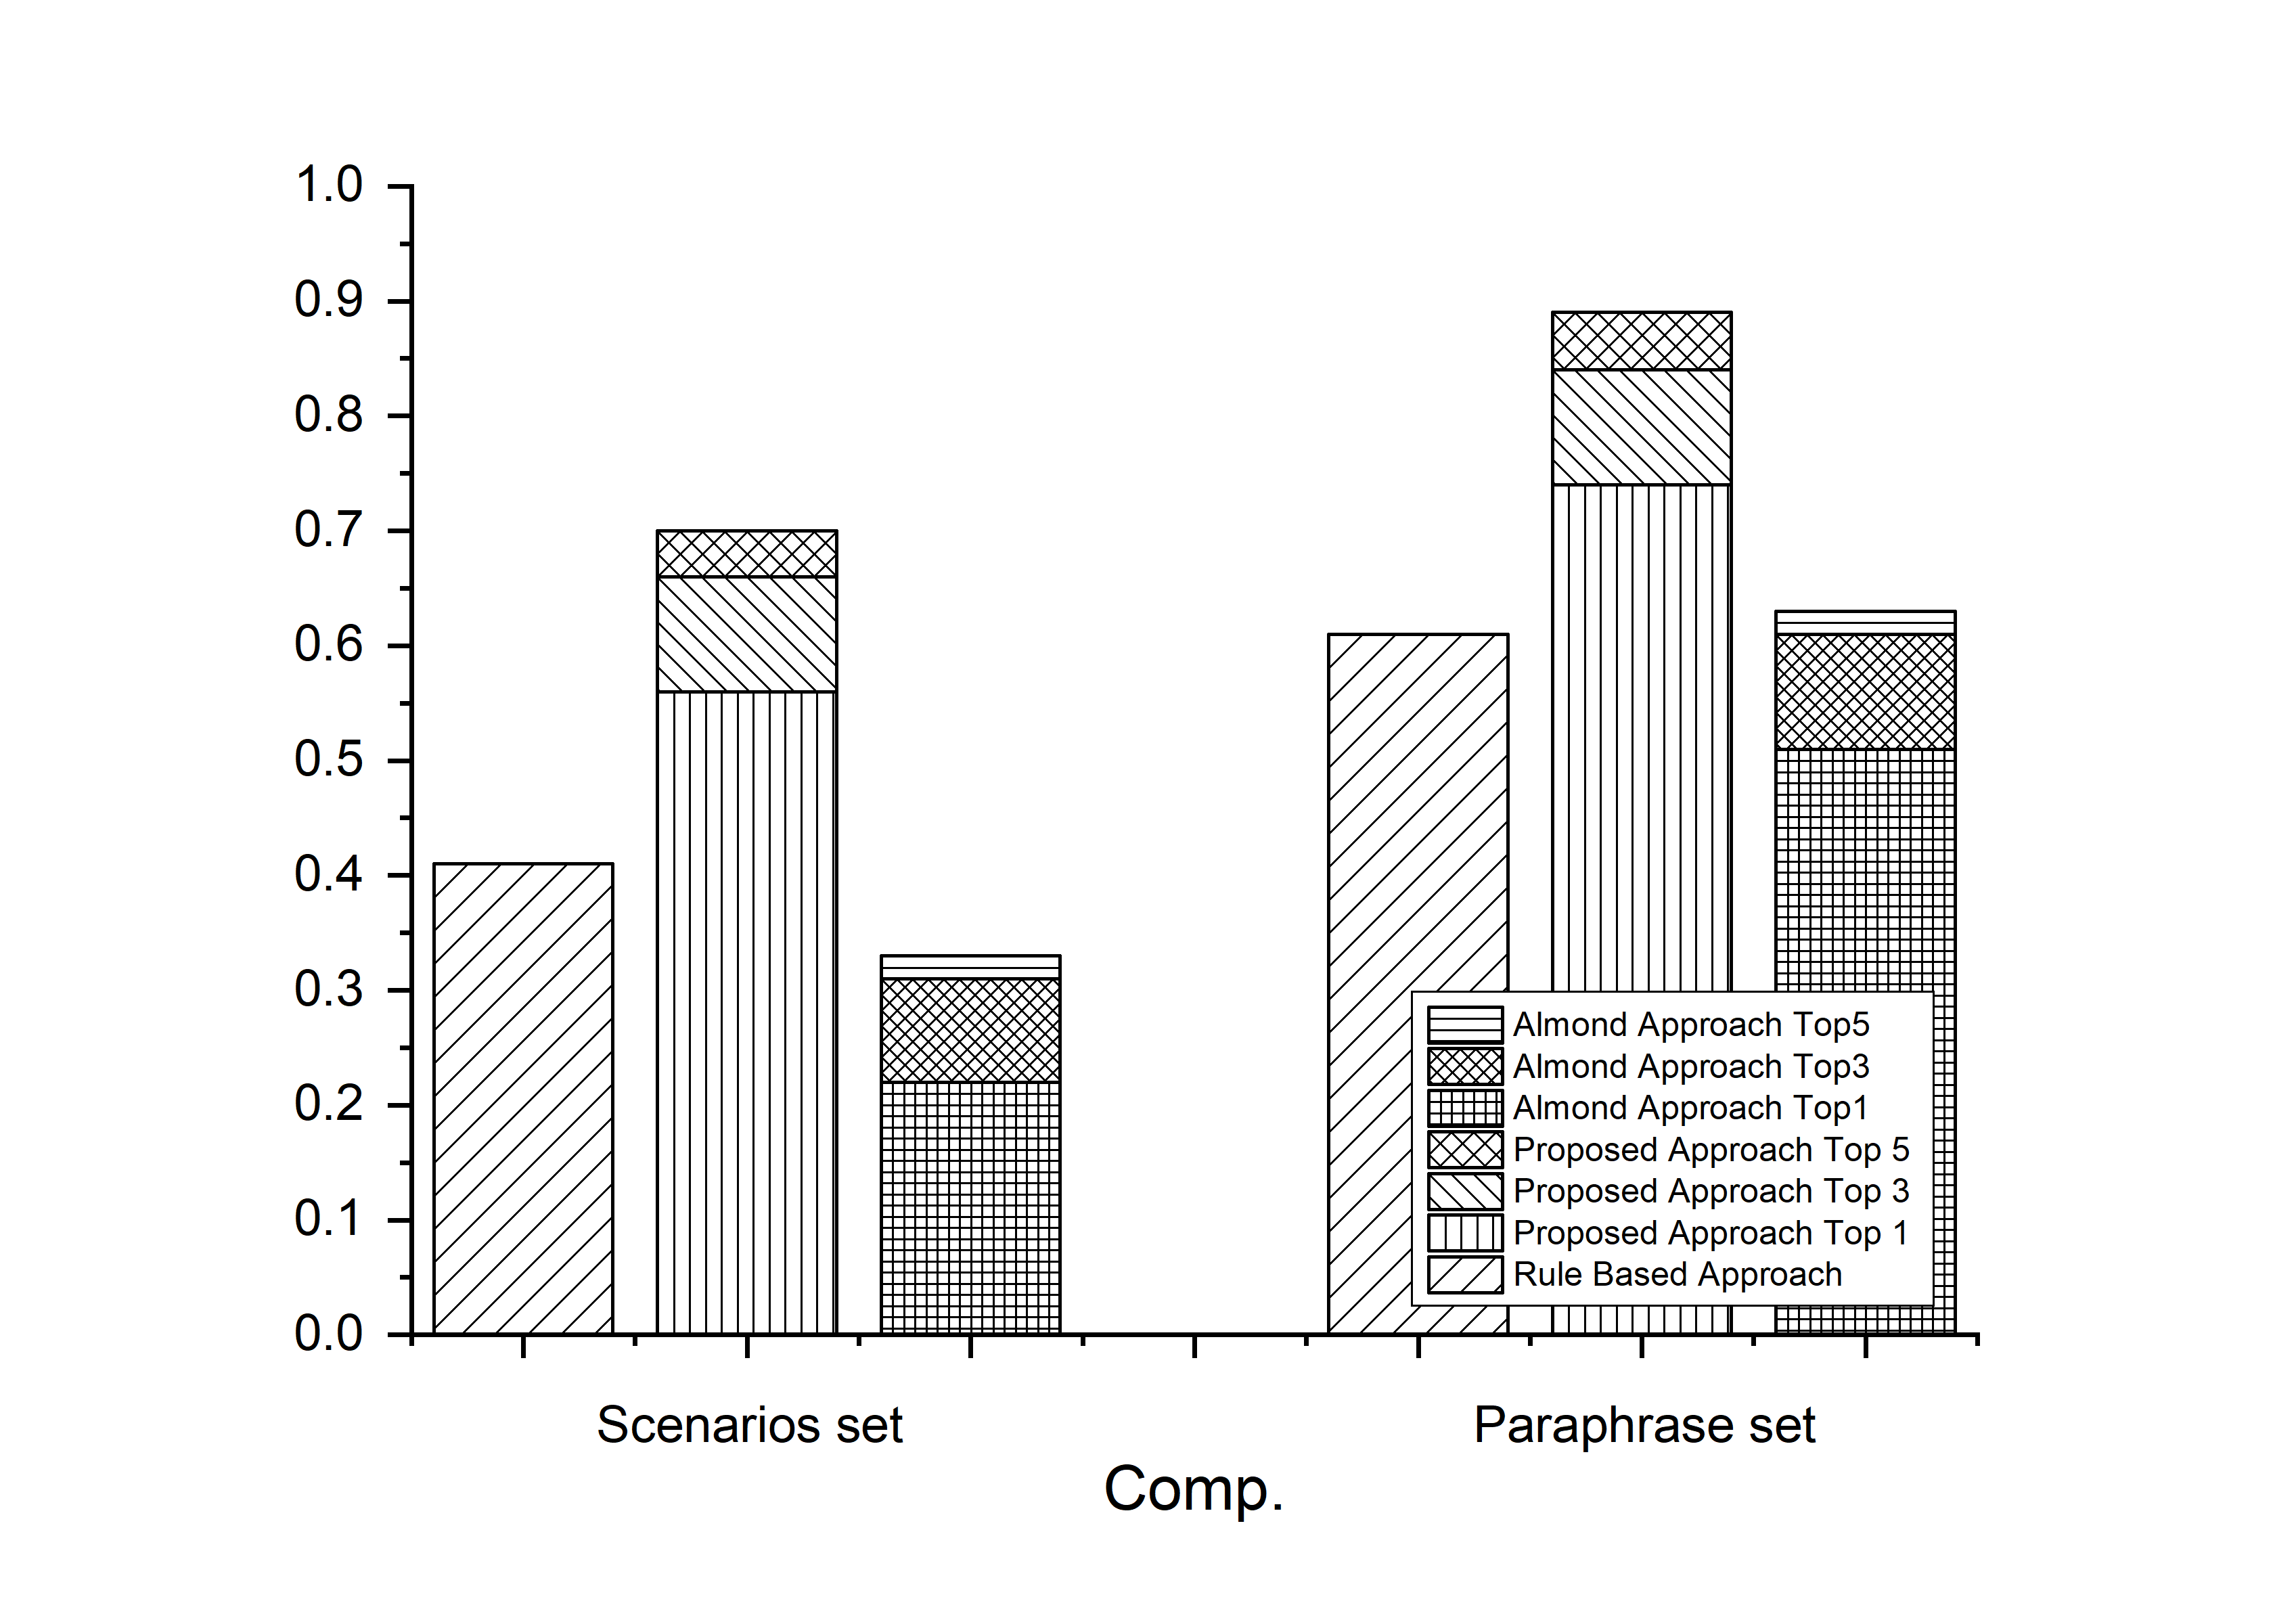
\includegraphics[width = .5\textwidth]{fig5_2.png}
\caption{Instructions Recognition Accuracy of Three Approaches}
\end{figure}
The experimental results are shown in Fig.5.The left shows the accuracy of recognition of the primitive instructions by rule based approach, our approach and Almond approach in the three sets. The right shows the accuracy of recognition of the compound instructions by rule based approach, our approach and Almond approach in the three sets.

In the Base set, the accuracy of the rule based approach, our approach and Almond approach are all 100\%. This is because the Base set is composed of instructions which are generated by the rules defined in Section 4.2. Therefore these approaches can accurately recognize these most basic instructions.

In the Paraphrase set, you can see that the accuracy of the rule based approach on the primitive instructions is 77\%. Because the rule based approach can only recognize the sentence structure and specification defined by rules in the text. Once the sentence structure or lexical representation becomes undefined ,the approach cannot recognize the instructions any more. The accuracy of the rule based approach in the recognition of compound sentences is only 61\%. Because the structure of compound instructions are too complex and diverse. If you need to recognize them accurately, you have to define a large number of rules for each type of sentence. It cannot be defined one by one obviously. For example, if the marker words of the condition in the compound sentence are not defined, the sentence structure will change and it will not be recognized. In our approach, the Top1 recognition accuracy of the primitive instructions is 86\%, Top3 is 91\%, and Top5 is 94\%. Our approach can solve the problem of sentence structure and partial word change. However, because of the limitations of the natural language processing method used in this paper, it still causes some groups of synonym to be unrecognizable, such as device operation "turn down" should be recognized as "reduce". However, it will match the "turn off" with higher similarity of the word vector in practice . Our approach obtained an accuracy of 74\% at Top 1 in the compound instructions, 84\% at Top3, and 89\% at Top5. Its recognition accuracy is about 5\%~12\% lower than primitive instructions. Because we split the compound instruction into two primitive instructions and matches separately. Then we synthesize the compound instructions according to the compound instructions combination strategy of 4.3 and it will display five matching results. In the matching of compound instructions, only the two primitive sentences that make up it match correctly, which can be correctly recognized. Therefore, it will make the accuracy to drop . In the Almond approach, the Top1 recognition accuracy of the primitive instructions is 77\%, Top3 is 88\%, Top5 is 89\%, the compound instructions Top1 recognition accuracy is 51\%, Top3 is 61\%, Top5 is 63\%. On the one hand, the Thingpedia of Almond is an open domain-based knowledge base. If you want to improve the accuracy of instructions in a specific field, you have to train in advance for that particular field, which requires extra work. On the other hand, because of the training of the Almond is not oriented to the smart home scenario, so the accuracy of the operation instructions directly to the device in this scenario is not as good as our approach.

In the Scenario set, There are more complex and colloquial instructions than Paraphrase set. It greatly increase the challenge of instruction recognition. The Scenario set contains many highly abstract instructions that make our approach and the other two approaches can not recognize the instruction. In primitive instructions, the accuracy of the rule based approach is 64\%. Our approach obtains an accuracy of 74\% in Top1, 81\% in Top3, 86\% in Top5. Almond approach obtained an accuracy of 34\% in Top1, 54\% in Top3 and 65\% in Top5.In compound Instructions, the accuracy of the rule based approach is 41\%, our approach obtains an accuracy of 56\% in Top1, 66\% in Top3, 70\% in Top5. Almond approach obtained an accuracy of 22\% in Top1, 31\% in Top3, 33\% in Top5. The reason for the low accuracy is mainly due to the volunteers' various semantic and complex instructions which based on their life experience and the given smart home scenario. For example, volunteers may give an abstract condition such as "if the sitting room is well lighted" when setting the room brightness service. At this time, the rule based approach, our approach and the Almond approach will not understand the semantics and recognize wrongly. However, our approach instruction recognition rate is higher than the other two approaches, because we define a series of “Context” entities on the knowledge graph which is based on the smart home scenario. So our approach can recognize some of the instructions with high-level semantics and then the instruction recognition accuracy is lower than the other two approaches. For example, for the living room air quality query "How is the air quality of the living room?", the rule based approach and the Almond approach cannot understand the specific meaning of "air quality", and our approach defines the “Context” of the concentration of PM2.5 in the living room. So we can know that this query instruction is asking about the air quality in the living room, and finally correctly matches the instruction "What is the PM2.5 in the sitting room ?". Then it will execute Get $C_i.CValue$ to get the concentration of PM2.5 in the living room air. 

In primitive instructions, the accuracy of the rule based approach is reduced by 14\% compared to the Paraphrase set. The accuracy of our approach is reduced by 8\% to 12\%, and the accuracy of the Almond approach is reduced by 24\% to 43\%; In compound instructions, the accuracy of the rule based approach is reduced by 23\% compared to the Paraphrase set, the accuracy of our approach is reduced by 18\% to 19\%, and the accuracy of the Almond approach is reduced by 29\% to 30\%.

This shows that in our “Context” entity which defined in the knowledge graph with scenario, it can really improve the recognition accuracy of some high-level semantic instructions in the smart home scenario.

In summary, our approach can not only recognizes instructions generated by rules, but also has a high recognition accuracy for instruction sets written by trained testers. It can also adapt to scenes to understand some more semantically complex instructions.

\subsection{Reduction for Lines of Code}

Table 12 displays the comparison of LOC between the two approaches for smart home situational awareness services . When using Java to develop these services, each service is developed independently. While using the approach of this paper, developers only need to implement scenario-oriented configuration, that is, the base code which has 115 lines. In the development for these service by Java, the codes of interface calls are the codes of underlying device interface calls. The approach of this paper only requires users to give instructions. Then the parser will parse through the underlying code. And we use the runtime knowledge graph to achieve the same function without adding any redundant code. For example, $S_{11}$ is Jack's temperature adjustment service, and the lines of code for the Java program are 220, where the codes of interface calls are 136 lines, the management logic codes are 84 lines. $S_{23}$ is Ken's air conditioning service, the Java program has 140 lines of code, wherein the interface call codes are 68 lines, management logic codes are 72 lines. The average lines of code for a Java program are 186 lines, and the average lines of code for the approach of this paper only require 10 lines. So the code reduction is over 94.8\%.

\begin{table}[h]
	\centering
	\begin{tabular}[h]{|c|c|c|c|c|c|c|c|c|c|c|c|c|c|c|c|}				
		\hline
		& Basic& $S_{11}$ & $S_{12}$ & $S_{13}$ & $S_{21}$ & $S_{22}$ & $S_{23}$ & $S_{31}$ & $S_{32}$& $S_{41}$ & $S_{42}$& $S_{51}$ & $S_{52}$&Average\\
		\hline
		Java & 0 & 220 & 198  & 140 & 220 & 198  & 140 & 220& 197  & 163 & 188& 163  & 188 & 220\\
		\hline
		Our Approach & 115 & 0 & 0 & 0 & 0 & 0& 0 & 0 & 0& 0 & 0 & 0 &0&10\\
		\hline		
	\end{tabular}
	\caption{Comparison in LOC of Two Approaches}	
\end{table}

\subsection{Program Execution Time}

\begin{figure}[h]
	\centering
	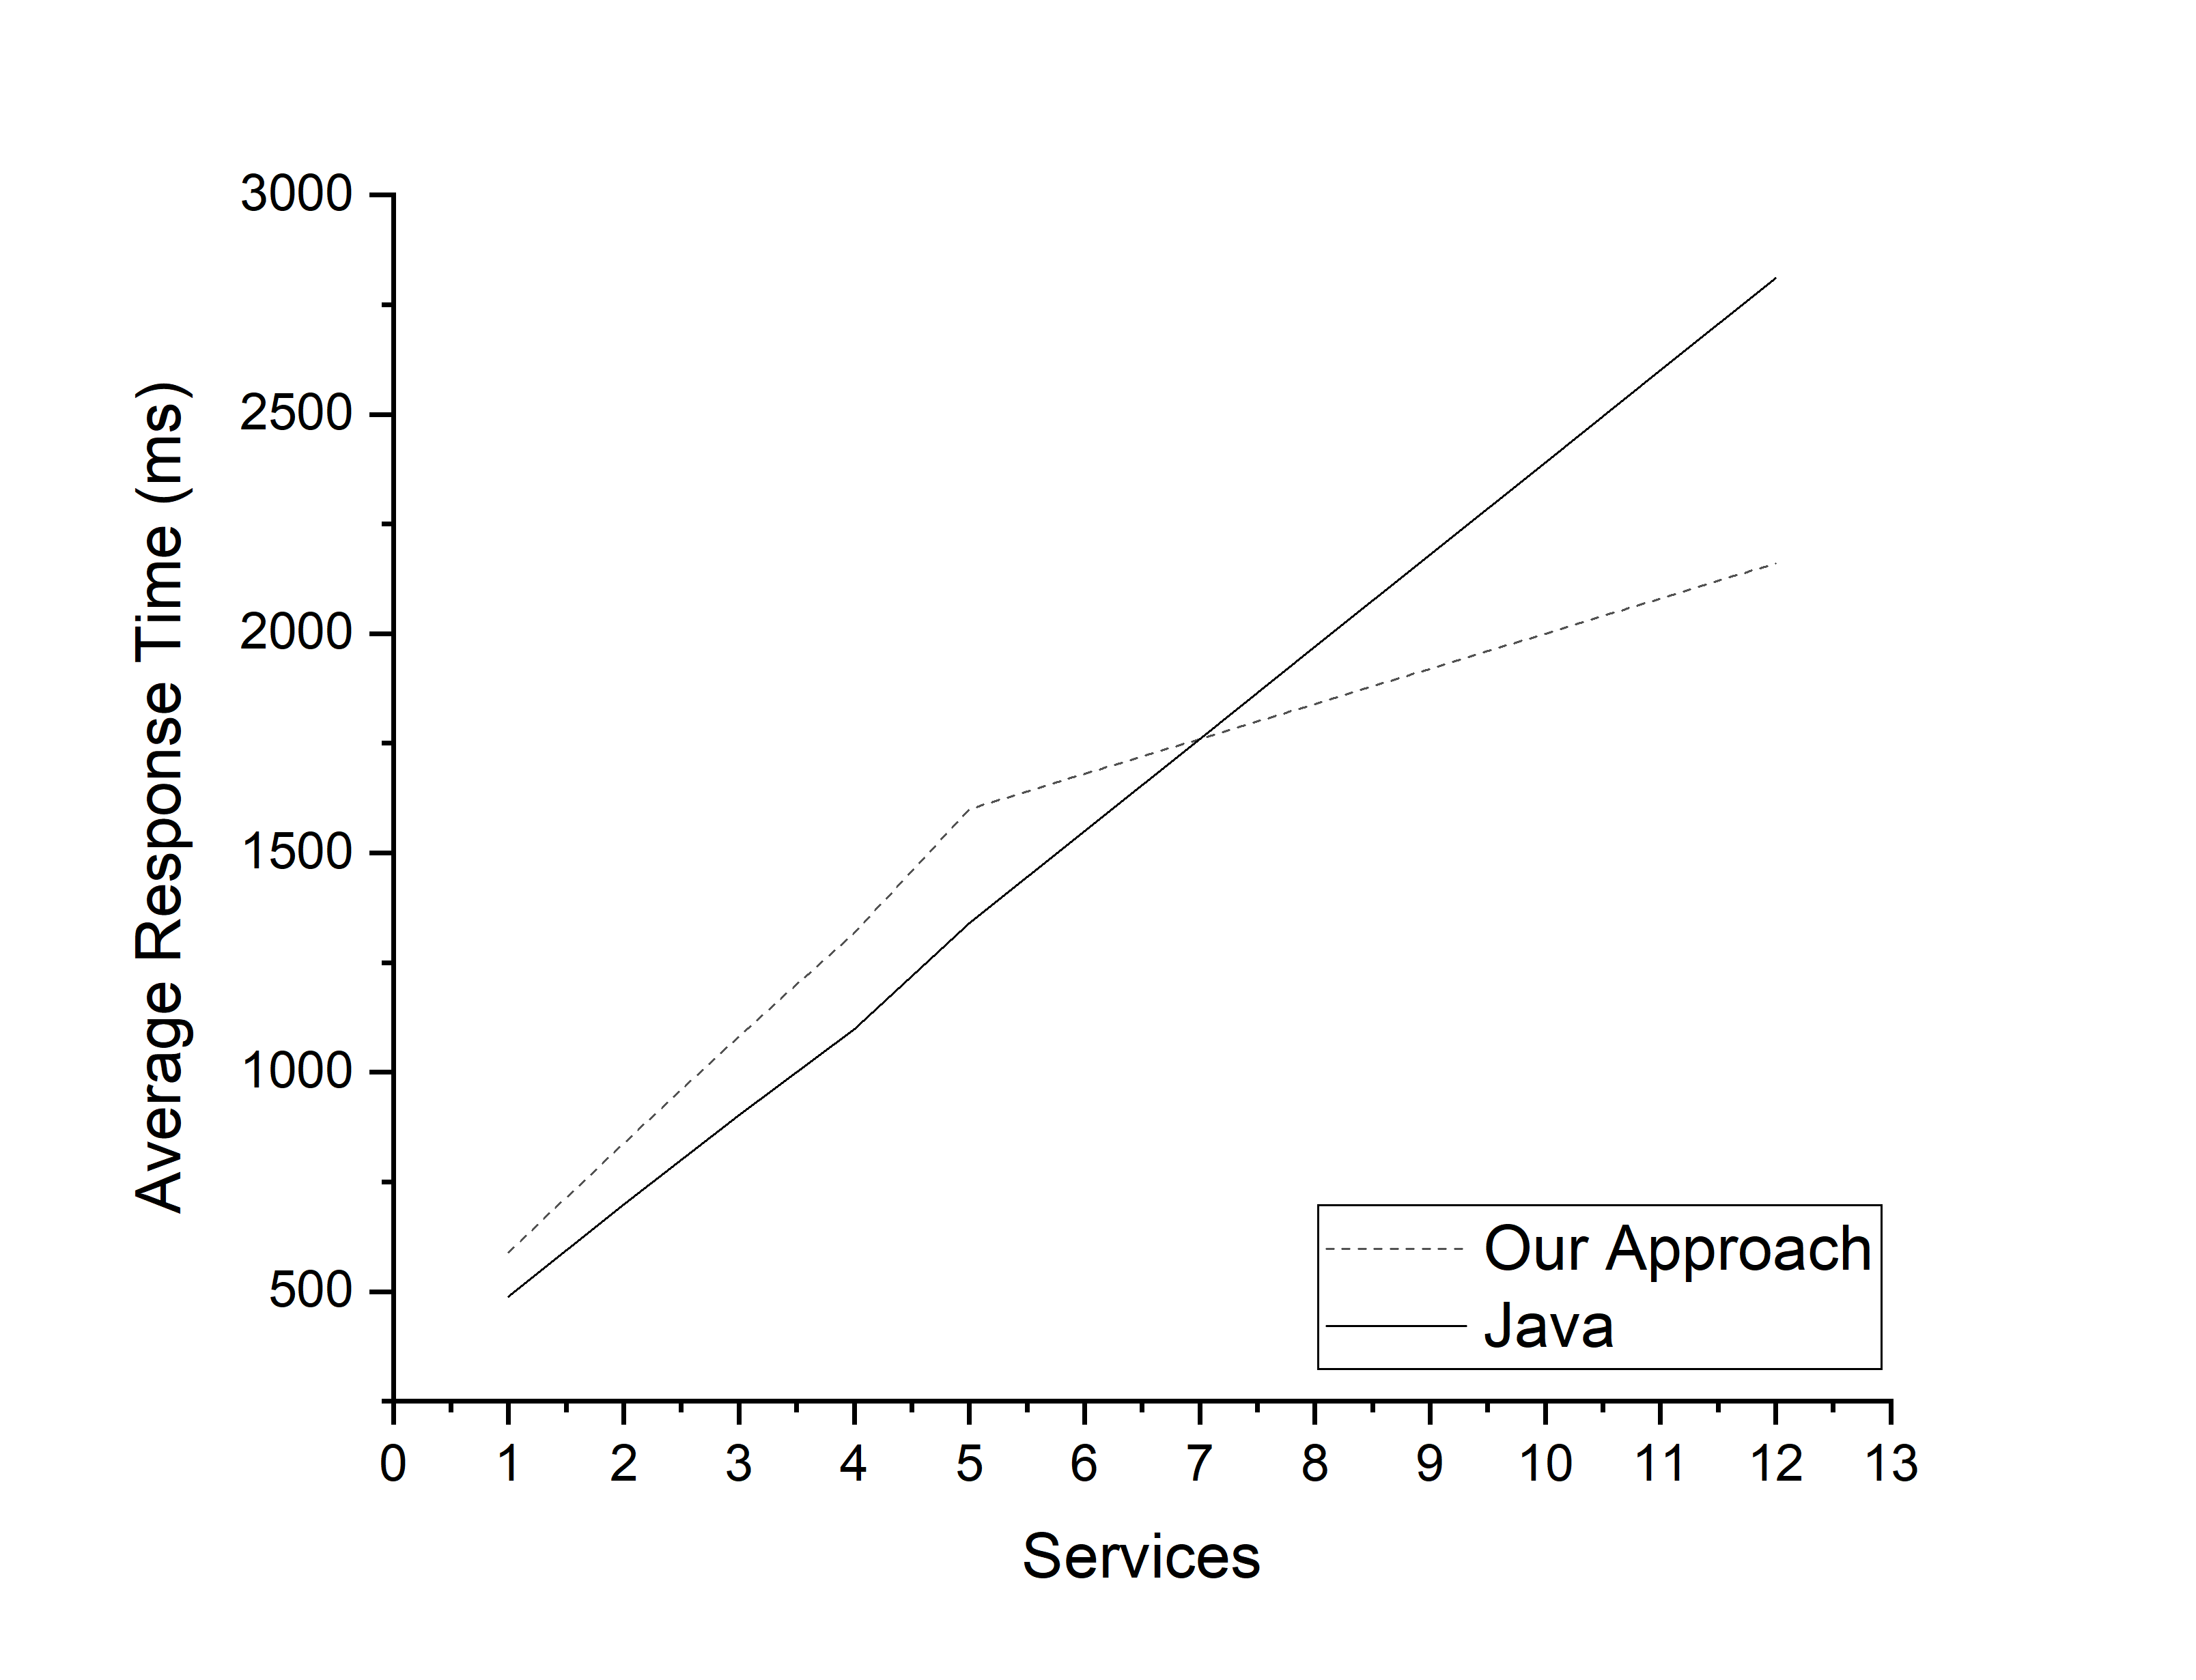
\includegraphics[width = .8\textwidth]{fig6.png}
	\caption{Comparison in Execution Time of Two Approaches}
\end{figure}

In order to compare the service execution performance between the two approaches. The development environment is a server with 3.1GHz 4Core CPU, 4GB RAM. Different numbers of smart home situational awareness services are executed. The average response time is counted,which is shown in Figure 6. In a Java program, each service is executed sequentially. The management logic is executed separately and the device APIs are called. Therefore, the average response time increases linearly with the number of services. When using the approach of this paper, the knowledge graph instance model is transformed by the model operation and the device API calls to realize two-way synchronization with real-time information of the scenario. On this basis, knowledge reasoning is performed according to service requirements. On the one hand, additional operations are needed to maintain the runtime synchronization of the instance model and the smart home scenarios. When the number of services is small, the average response time of this approach is higher than Java programs. For the perspective of intelligent services, this difference in performance is acceptable. On the other hand, the services in the Java program are executed independently, when the service reaches a certain number, so there will be cases that different context aware services call the same device API to obtain scene information (for example, $C_{11}$, $C_{21}$ and $C_{31}$ are all to monitor the living room temperature). When there is a large number of services,the proposed approach can effectively reduce the overhead equipment API called repeatedly generated so that the average response time is low.



\section{Related Work}\label{sec:relatedwork}
\input{relatedwork}
\section{Conclusion}\label{sec:conclusion}
\input{conclusion}

\bibliography{reference}
\bibliographystyle{splncs04}


% \end{thebibliography}
\end{document}
